\documentclass[11pt]{article}
\usepackage[margin=1.1in]{geometry}
\usepackage{amsmath,amssymb,amsthm}
\usepackage{enumitem}
\usepackage{tikz}
\usetikzlibrary{automata,positioning,arrows.meta}
\usepackage[colorlinks=true,linkcolor=blue!50!black,citecolor=blue!50!black,urlcolor=blue!50!black]{hyperref}

\newtheorem{theorem}{Theorem}[section]
\newtheorem{lemma}[theorem]{Lemma}
\newtheorem{proposition}[theorem]{Proposition}
\newtheorem{corollary}[theorem]{Corollary}
\newtheorem{claim}[theorem]{Claim}
\theoremstyle{definition}
\newtheorem{definition}[theorem]{Definition}
\newtheorem{remark}[theorem]{Remark}
\newtheorem{example}[theorem]{Example}

\newcommand{\AN}{A_N}
\newcommand{\ANe}{A_{Ne}}
\newcommand{\N}{\mathbb{N}}
\newcommand{\Z}{\mathbb{Z}}
\DeclareMathOperator{\lcm}{lcm}

\title{Exact beats unique infinitely often:\\
a separation of nondeterministic automatic complexities}
\author{}
\date{August 24, 2026}

\begin{document}
\maketitle

\begin{abstract}
Let $\AN(w)$ denote the unique nondeterministic automatic complexity of a word
$w$ (the least number of states of an NFA accepting $w$ by a \emph{unique}
accepting path among inputs of length $|w|$), and let $\ANe(w)$ denote the
exact nondeterministic automatic complexity (the least number of states of an
NFA accepting $w$ and \emph{no other word} of length $|w|$, multiple accepting
paths allowed), as introduced by Chen, Kjos-Hanssen, Koswara, Richter and
Stephan (FSTTCS 2025), who asked whether the two measures ever differ. The word
$w_0=0123333333340156$ separates them: $\ANe(w_0)\le 8<9=\AN(w_0)$. We prove that
the separation occurs infinitely often, and in the strongest sense: for every
$k\equiv 0 \pmod 3$, $k\ge 3$, the word
\[
z_k \;=\; a_1a_2\cdots a_k\, b^{\,k+5}\, c\, a_1a_2\cdots a_{k-1}\, d\,e
\]
of length $3k+7$ over an alphabet of $k+4$ letters satisfies
$\ANe(z_k)\le k+5 < k+6 = \AN(z_k)$. Here $z_3$ is $w_0$ up to renaming of
letters. Consequently every minimum-size exact acceptor of $z_k$ has at least
two accepting paths. The upper bounds are by explicit machines; the lower
bound $\AN(z_k)\ge k+6$ is proved by a structural analysis of uniquely
accepting walks, whose main tools --- a splicing lemma, a rotation lemma, and a
two-visit lemma derived from the square structure of $z_k$ --- may be of
independent interest. All constructions and all instances $k\le 18$ of the
lower bound have additionally been verified by exhaustive computer search.
\end{abstract}

\section{Introduction}

Automatic complexity, introduced by Shallit and Wang \cite{SW} and developed
nondeterministically by Hyde and Kjos-Hanssen \cite{HK}, measures the size of
the smallest finite automaton that singles out a word $w$ among all words of
its length. In the nondeterministic setting two natural formalizations
coexist. Following the terminology of Chen, Kjos-Hanssen, Koswara, Richter and
Stephan \cite{CKKRS}:

\begin{definition}\label{def:complexities}
Let $w$ be a word of length $n$ over an alphabet $\Sigma$. An NFA $M$
(with a single start state, no $\varepsilon$-transitions) \emph{exactly
accepts} $w$ if $L(M)\cap\Sigma^{n}=\{w\}$. It \emph{uniquely accepts} $w$ if
moreover $M$ has exactly one accepting computation path of length $n$.
The \emph{exact nondeterministic automatic complexity} $\ANe(w)$ is the least
number of states of an NFA exactly accepting $w$; the \emph{unique
nondeterministic automatic complexity} $\AN(w)$ is the least number of states
of an NFA uniquely accepting $w$.
\end{definition}

Since unique acceptance implies exact acceptance, $\ANe(w)\le\AN(w)$ for every
$w$. Whether the inequality can be strict was raised in \cite{CKKRS} as the
``cardinal open question'' about the impact of exactness. The word
\[
w_0 \;=\; 0\,1\,2\,3^8\,4\,0\,1\,5\,6 \qquad (|w_0|=16)
\]
answers it: there is an $8$-state NFA exactly accepting $w_0$
(Figure~\ref{fig:M3}), while an exhaustive search shows that no $8$-state NFA
uniquely accepts $w_0$; thus $\ANe(w_0)\le 8<9=\AN(w_0)$, and every $8$-state
exact acceptor of $w_0$ has more than one accepting path.

A single example leaves open whether the phenomenon is sporadic. Renaming
letters injectively produces infinitely many words with the same property, but
these are all copies of $w_0$; the substantive question is whether there are
infinitely many words that are pairwise distinct up to renaming --- for
instance, of unbounded length. In this paper we prove that there are.

\begin{theorem}[Main Theorem]\label{thm:main}
For every $k\ge 3$ with $k\equiv 0\pmod 3$, let
\[
z_k \;=\; a_1a_2\cdots a_k \; b^{\,m}\; c \; a_1a_2\cdots a_{k-1}\; d\, e,
\qquad m=k+5,\quad n:=|z_k|=3k+7,
\]
over the alphabet $\Sigma_k=\{a_1,\dots,a_k,b,c,d,e\}$ of $k+4$ letters. Then
\[
\ANe(z_k)\;\le\;k+5\;<\;k+6\;=\;\AN(z_k).
\]
\end{theorem}

\begin{corollary}\label{cor:inf}
There are infinitely many words $w$, of unbounded length and pairwise distinct
up to renaming of letters, with $\ANe(w)<\AN(w)$.
\end{corollary}

\begin{corollary}\label{cor:paths}
For every such $k$, every $(k+5)$-state NFA exactly accepting $z_k$ has at
least two accepting paths spelling $z_k$. (If some such NFA had a unique
accepting path it would witness $\AN(z_k)\le k+5$.)
\end{corollary}

Note that $z_3=a_1a_2a_3\,b^8\,c\,a_1a_2\,d\,e$ is precisely $w_0$ under the
renaming $a_1a_2a_3\mapsto 012$, $b\mapsto3$, $c\mapsto 4$, $d\mapsto5$,
$e\mapsto6$; the family grows the free prefix, the folded suffix and the
run in lockstep. The congruence $k\equiv0\pmod 3$ (equivalently
$m\equiv2\pmod3$) is essential: for $k\not\equiv0\pmod 3$ a deterministic
three-state ``run gadget'' exists and collapses $\AN$ to $k+5$, destroying the
separation. This modular obstruction is the heart of the lower bound.

The proof of the upper bound $\ANe(z_k)\le k+5$ is an explicit construction
(Section~\ref{sec:upper}). The lower bound $\AN(z_k)\ge k+6$ occupies
Sections~\ref{sec:tools}--\ref{sec:endgame}. It proceeds by the walk
characterization of unique acceptance (Section~\ref{sec:prelim}) and four
master lemmas: a \emph{splicing lemma} (any second same-length path between
two time-compatible states of the accepting walk contradicts uniqueness), a
\emph{rotation lemma} (two state-coincidences at equal time-shifts force
edge-level periodicity), a \emph{two-visit lemma} (a state visited three
times forces a square in $z_k$, which the word forbids outside its unary run),
and a \emph{crossing lemma} (two crossing coincidences of states allow the
three blocks of the walk between them to be exchanged, $XYZ\mapsto ZYX$,
producing a second accepting path unless the exchange is invisible).
The two-visit lemma confines all cycling of a hypothetical small walk to a
cluster of at most four states carrying a single cycle $\gamma$; every
second path is then assembled from segments of the walk joined at
coincidences, with the number of turns around $\gamma$ used as a free
parameter to adjust lengths. A counting argument forces a nonempty aligned
fold of the suffix onto the prefix, the crossing lemma pins every remaining
coincidence to one of a few positions relative to the fold, and a case
analysis on the length $\ell\in\{1,2,4\}$ of $\gamma$ --- $\ell=3$ being
excluded precisely by the hypothesis $m\equiv2\pmod 3$ --- eliminates every
configuration by an explicit second path. The argument is uniform in $k$;
only the smallest cases $k\le15$ are delegated to a computer.

The base case $k=3$ and the instances $k=6,9,12,15,18$ of the lower bound
have been verified by an exhaustive, pruned search over all
uniquely-accepting walks (Section~\ref{sec:verification}); the proof for
$k\ge18$ is self-contained, so the instance $k=18$ is confirmed twice. All constructions of the paper, and the individual surgeries
of the lower-bound proof, have additionally been machine-checked.

\begin{remark}
The levels of both complexities are, for each fixed alphabet and state bound
$q$, regular languages: for a fixed NFA $M$ the set of lengths $n$ such that
$|L(M)\cap\Sigma^n|=1$ (respectively, such that $M$ has exactly one accepting
path of length $n$) is eventually periodic, and
$\{w:\ANe(w)\le q\}$, $\{w:\AN(w)\le q\}$ are finite unions over the finitely
many $q$-state machines of intersections of regular languages with such length
sets. Thus $\{w : \ANe(w)\le q<\AN(w)\}$ is regular, and
Theorem~\ref{thm:main} may be read as saying that these ``gap languages'' are
nonempty for infinitely many parameters. Our proof gives explicit witnesses
rather than pumping abstractly, since regularity alone does not decide
infinitude at a fixed level.
\end{remark}

\section{Preliminaries: unique acceptance and walks}\label{sec:prelim}

Fix a word $z$ of length $n$ over $\Sigma$. An NFA is a tuple
$M=(Q,\Sigma,\Delta,q_0,F)$ with $\Delta\subseteq Q\times\Sigma\times Q$. A
\emph{path} of length $t$ is a sequence of transitions
$(p_0,x_1,p_1)(p_1,x_2,p_2)\cdots(p_{t-1},x_t,p_t)\in\Delta^t$; it
\emph{spells} $x_1\cdots x_t$. An accepting path of length $n$ is one with
$p_0=q_0$ and $p_n\in F$.

Unique acceptance has a purely combinatorial normal form. Call a coloring
$c_0,c_1,\dots,c_n$ of the positions $0,\dots,n$ by states, together with the
induced \emph{walk graph}
\[
\Delta_W=\{\,e_t:=(c_t,z_t,c_{t+1})\;:\;0\le t\le n-1\,\}
\]
(a set of transitions; repetitions merge), a \emph{uniquely accepting walk}
for $z$ if the NFA $(\{c_0,\dots,c_n\},\Sigma,\Delta_W,c_0,\{c_n\})$ has
exactly one path of length $n$ from $c_0$ to $c_n$. (That path is then
necessarily $e_0e_1\cdots e_{n-1}$, which spells $z$; so this NFA uniquely
accepts $z$.)

\begin{lemma}[Walk characterization]\label{lem:walk}
$\AN(z)$ is the least number of distinct states of a uniquely accepting walk
for $z$.
\end{lemma}

\begin{proof}
A uniquely accepting walk with $s$ states is an NFA with $s$ states uniquely
accepting $z$, so $\AN(z)\le s$. Conversely let $M$ uniquely accept $z$ with
$\AN(z)$ states and let $P=e_0\cdots e_{n-1}$ be its unique accepting path,
visiting states $c_0,\dots,c_n$. Delete all states and transitions of $M$ not
on $P$, and shrink $F$ to $\{c_n\}$. Deletion cannot create accepting paths
and $P$ survives, so the trimmed automaton still uniquely accepts $z$; its
transition set is exactly $\{e_t\}$ and its states are $\{c_0,\dots,c_n\}$.
Thus the coloring $c_0,\dots,c_n$ is a uniquely accepting walk with at most
$\AN(z)$ states.
\end{proof}

Throughout the lower-bound proof we therefore work with a hypothetical
uniquely accepting walk $W=(c_0,\dots,c_n)$ for $z=z_k$ and write
$Q=\{c_0,\dots,c_n\}$, $e_t=(c_t,z_t,c_{t+1})$, and $W[i,j]=e_ie_{i+1}\cdots
e_{j-1}$ (a path from $c_i$ to $c_j$ of length $j-i$). A \emph{visit} of a
state $s$ is a time $t\in\{0,\dots,n\}$ with $c_t=s$.

We record the position structure of $z_k$. Letters $a_1,\dots,a_{k-1}$ occur
twice, at positions $i-1$ and $\delta_0+(i-1)$ where
\[
\delta_0:=2k+6;
\]
letters $a_k$ (position $k-1$), $c$ (position $2k+5$), $d$ (position $3k+5$)
and $e$ (position $3k+6$) occur once; letter $b$ occupies exactly the
positions $k,\dots,2k+4$ ($m=k+5$ of them). We call
$[k,\,2k+5]$ the \emph{run window}: the states $v_j:=c_{k+j}$
($0\le j\le m$) are the \emph{run states}, visited at the \emph{run times}
$k,\dots,2k+5$. The remaining times are the \emph{prefix times} $[0,k-1]$
(states $g_j:=c_j$; also write $g_k:=c_k=v_0$) and the \emph{tail times}
$[2k+6,\,3k+7]$ (states $h_j:=c_{2k+6+j}$ for $0\le j\le k-1$, then
$u_1:=c_{3k+5+1}=c_{3k+6}$ and $u_2:=c_n$). There are $n+1=3k+8$ times in all:
$k$ prefix times, $k+6$ run times, and $k+2$ tail times.

\section{The upper bounds}\label{sec:upper}

\subsection{An exact acceptor with \texorpdfstring{$k+5$}{k+5} states}

\begin{figure}[t]
\centering
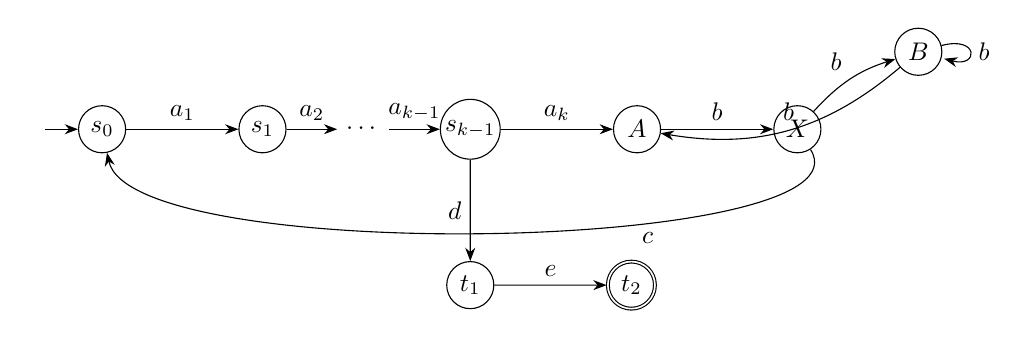
\begin{tikzpicture}[->,>=Stealth,node distance=1.55cm,every state/.style={minimum size=6.5mm,inner sep=1pt},scale=0.92,transform shape]
\node[state,initial,initial text={}] (s0) {$s_0$};
\node[state,right=of s0] (s1) {$s_1$};
\node[right=0.7cm of s1] (dots) {$\cdots$};
\node[state,right=0.7cm of dots] (sk1) {$s_{k-1}$};
\node[state,right=of sk1] (A) {$A$};
\node[state,right=of A] (X) {$X$};
\node[state,above right=0.6cm and 1.2cm of X] (B) {$B$};
\node[state,below=1.4cm of sk1] (t1) {$t_1$};
\node[state,accepting,right=of t1] (t2) {$t_2$};
\path (s0) edge node[above] {$a_1$} (s1)
      (s1) edge node[above] {$a_2$} (dots)
      (dots) edge node[above] {$a_{k-1}$} (sk1)
      (sk1) edge node[above] {$a_k$} (A)
      (A) edge node[above] {$b$} (X)
      (X) edge[bend left=15] node[above left] {$b$} (B)
      (B) edge[bend left=25] node[above] {$b$} (A)
      (B) edge[loop right] node[right] {$b$} (B)
      (sk1) edge node[left] {$d$} (t1)
      (t1) edge node[above] {$e$} (t2);
\draw[->] (X) .. controls +(1.1,-1.7) and +(0.4,-1.9) .. node[below,pos=0.35] {$c$} (s0);
\end{tikzpicture}
\caption{The exact acceptor $M_k$ ($k+5$ states). For $k=3$ this is an
$8$-state NFA exactly accepting $w_0=0123^8\,40156$, with three accepting
paths.}\label{fig:M3}
\end{figure}

Define the NFA $M_k$ with states
$s_0,\dots,s_{k-1},A,X,B,t_1,t_2$ ($k+5$ states), start $s_0$, final
$\{t_2\}$, and transitions
\[
\begin{array}{llll}
s_{i-1}\xrightarrow{\,a_i\,}s_i\ (1\le i\le k-1), &
s_{k-1}\xrightarrow{\,a_k\,}A, &
s_{k-1}\xrightarrow{\,d\,}t_1, &
t_1\xrightarrow{\,e\,}t_2,\\[2pt]
A\xrightarrow{\,b\,}X, &
X\xrightarrow{\,b\,}B, &
B\xrightarrow{\,b\,}A,\quad B\xrightarrow{\,b\,}B, &
X\xrightarrow{\,c\,}s_0 .
\end{array}
\]

\begin{lemma}\label{lem:gadgetT}
The set of lengths of paths from $A$ to $X$ in the $b$-labelled subgraph of
$M_k$ is $T=\{1\}\cup\{t\in\N: t\ge4\}$. For $t\ge 8$ there are at least
three such paths of length $t$.
\end{lemma}

\begin{proof}
Any $b$-path from $A$ to $X$ decomposes as the edge $A\to X$ followed by a
number $r\ge0$ of returns $X\to B\to B^{j}\to A\to X$ of lengths $3+j$
($j\ge0$). Hence its length is $1+\sum_{i=1}^r(3+j_i)$, and the achievable
lengths are $\{1\}\cup[4,\infty)$. The number of paths of length $t$ is the
number of ordered compositions of $t-1$ into parts $\ge3$; for $t\ge8$,
$t-1\ge7$ has at least the compositions $(t-1)$, $(3,t-4)$, $(t-4,3)$.
\end{proof}

\begin{proposition}\label{prop:upper-exact}
$M_k$ exactly accepts $z_k$ for every $k\ge3$ (no congruence needed). Hence
$\ANe(z_k)\le k+5$, and $M_k$ has at least three accepting paths.
\end{proposition}

\begin{proof}
First, $z_k\in L(M_k)$ via
$s_0\cdots s_{k-1}\,A\,(b\text{-path of length }m)\,X\,s_0\cdots
s_{k-1}\,t_1\,t_2$, using $m=k+5\ge 8\in T$; by Lemma~\ref{lem:gadgetT} there
are at least three such paths.

Conversely let $\pi$ be any accepting path of length $n$. The state $t_2$ has
no outgoing transitions and only the incoming $e$-transition from $t_1$; $t_1$
only the incoming $d$-transition from $s_{k-1}$; and $s_{k-1}$ is reachable
only along the chain $s_0\to\cdots\to s_{k-1}$ spelling $a_1\cdots a_{k-1}$,
whose sole entry point $s_0$ is entered only by the $c$-transition from $X$
(or is the start). Likewise $A$ is entered only from $s_{k-1}$ by $a_k$, and
$X$ only by $b$-transitions from within the gadget. It follows that $\pi$ has
the shape
\[
\Big(\;s_0\to\cdots\to s_{k-1}\xrightarrow{a_k}A
\xrightarrow{\,b^{t_i}\,}X\xrightarrow{c}s_0\;\Big)_{i=1,\dots,r}\;
s_0\to\cdots\to s_{k-1}\xrightarrow{d}t_1\xrightarrow{e}t_2
\]
for some $r\ge0$ and $t_1',\dots,t_r'\in T$ (we write $t_i$ for the run
lengths), spelling
$\big(\prod_{i=1}^{r} a_1\cdots a_k\,b^{t_i}\,c\big)\,a_1\cdots a_{k-1}\,d\,e$,
of length $\sum_{i=1}^r\big((k+1)+t_i\big)+(k+1)$. Setting this equal to
$n=3k+7$ gives
\[
\sum_{i=1}^r t_i \;=\; (2-r)(k+1)+4 .
\]
For $r=1$: $\sum t_i=k+5=m\in T$, and the word spelled is $z_k$. For $r=2$:
$\sum t_i=4$, impossible since two elements of $T=\{1\}\cup[4,\infty)$ sum to
$2$ or to at least $5$, never to $4$. For $r\ge3$ the right-hand side is
negative, and $r=0$ gives length $k+1\ne n$. So every accepting path spells
$z_k$.
\end{proof}

\subsection{A unique acceptor with \texorpdfstring{$k+6$}{k+6} states}

\begin{proposition}\label{prop:upper-unique}
Let $D_k$ be the NFA with states $s_0,\dots,s_{k-1},A,x_1,x_2,x_3,t_1,t_2$
($k+6$ states), start $s_0$, final $\{t_2\}$, and transitions
\[
s_{i-1}\xrightarrow{a_i}s_i\ (i<k),\quad
s_{k-1}\xrightarrow{a_k}A,\quad
A\xrightarrow{b}A,\quad
A\xrightarrow{b}x_1\xrightarrow{b}x_2\xrightarrow{b}x_3
\xrightarrow{c}s_0,\quad
s_{k-1}\xrightarrow{d}t_1\xrightarrow{e}t_2 .
\]
Then $D_k$ uniquely accepts $z_k$. Hence $\AN(z_k)\le k+6$.
\end{proposition}

\begin{proof}
The set of $b$-path lengths from $A$ to $x_3$ is $T'=[3,\infty)$, each length
achieved by exactly one path (the number of loops at $A$ is determined). As in
Proposition~\ref{prop:upper-exact}, every accepting path of length $n$ has the
block shape with run lengths $t_i\in T'$ and $\sum_i t_i=(2-r)(k+1)+4$; now
$r=2$ requires $\sum t_i=4<3+3$, impossible, $r\ge3$ is negative, and $r=1$
forces $t_1=m$, realized by exactly one path. So $D_k$ has exactly one
accepting path, which spells $z_k$.
\end{proof}

\begin{remark}\label{rem:why-mod3}
Replacing the loop-plus-escape of $D_k$ by a $3$-cycle with entry--exit offset
$d\in\{0,1,2\}$ yields a $(k+5)$-state \emph{unique} acceptor whenever
$m\equiv d\pmod 3$ for some $d$ with the block equation
$\sum t_i=(2-r)(k+1)+4$ unsolvable in $T=\{d+3j\}$. For $m\equiv0,1\pmod3$
such offsets exist, and indeed the analogues of $z_k$ with
$k\not\equiv0\pmod3$ satisfy $\AN=k+5=\ANe$, as exhaustive search
confirms for small $k$; for $m\equiv2\pmod 3$ the
only offset with $m\in T$ is $d=2$, and then $t_1=t_2=2$ solves the $r=2$
equation, producing a second accepting path. This is the arithmetic seed of
the lower bound.
\end{remark}

\section{Master lemmas for the lower bound}\label{sec:tools}

For the rest of the paper fix $k\equiv0\pmod3$, $k\ge3$, write $z=z_k$,
$m=k+5\equiv2\pmod3$, $n=3k+7$, $\delta_0=2k+6$, and let
$W=(c_0,\dots,c_n)$ be a uniquely accepting walk for $z$ with state set $Q$.
We must show $|Q|\ge k+6$; suppose for contradiction $|Q|\le k+5$.

\begin{lemma}[Splicing]\label{lem:splice}
For all $0\le i\le j\le n$, the walk segment $W[i,j]$ is the \emph{only} path
of length $j-i$ from $c_i$ to $c_j$ in the walk graph.
\end{lemma}

\begin{proof}
If $\pi\ne W[i,j]$ were another such path, then $W[0,i]\,\pi\,W[j,n]$ would be
an accepting path of length $n$ different from $W[0,n]$.
\end{proof}

\begin{lemma}[Rotation]\label{lem:rotation}
Suppose $c_i=c_{i+\delta}$ and $c_p=c_{p+\delta}$ with $i<p$ and $\delta\ge1$.
Then $e_t=e_{t+\delta}$ for all $i\le t<p$. In particular
$z_t=z_{t+\delta}$ and $c_t=c_{t+\delta}$ for all $i\le t\le p$.
\end{lemma}

\begin{proof}
The path $\pi=W[0,i]\;W[i+\delta,\,p+\delta]\;W[p,n]$ is well defined
(junctions $c_i=c_{i+\delta}$ and $c_{p+\delta}=c_p$), accepting, and of
length $i+(p-i)+(n-p)=n$. By uniqueness $\pi=W[0,n]$ as edge sequences.
Comparing the edges at positions $t\in[i,p)$ gives $e_t=e_{t+\delta}$.
\end{proof}

\begin{lemma}[Pair table]\label{lem:pairs}
Let $\delta\ge1$ and $P_\delta=\{t: z_t=z_{t+\delta}\}$. Then
$P_{\delta_0}\supseteq[0,k-2]$ and, for $\delta\neq\delta_0$,
$P_\delta=[k,\,2k+4-\delta]$ (empty if $\delta>k+4$); moreover
$P_{\delta_0}=[0,k-2]$.
\end{lemma}

\begin{proof}
Equal letters at distance $\delta$ are either two $b$'s (both positions in
$[k,2k+4]$) or the two occurrences of some $a_i$ ($i\le k-1$), which are at
distance exactly $\delta_0$. Since $\delta_0=2k+6>k+4$, the two cases do not
mix. For $\delta=\delta_0$: $z_t=z_{t+\delta_0}$ holds iff $t\le k-2$
(at $t=k-1$: $a_k\ne d$; at $t=k$: $b\ne e$; $t>k$ is out of range).
\end{proof}

\begin{corollary}[Shift classification]\label{cor:shifts}
Call a pair $(i,i+\delta)$ with $c_i=c_{i+\delta}$ a \emph{$\delta$-chord}.
If two distinct $\delta$-chords exist for the same $\delta$, with earlier
starting points $i<p$, then Lemma~\ref{lem:rotation} and
Lemma~\ref{lem:pairs} force: either $\delta=\delta_0$ and $[i,p]\subseteq
[0,k-1]$, or both chords lie in the run window,
$[i,\,p+\delta]\subseteq[k,\,2k+5]$.
\end{corollary}

\begin{proof}
Rotation gives $z_t=z_{t+\delta}$ for $t\in[i,p)$, so $[i,p)\subseteq
P_\delta$. If $\delta\ne\delta_0$ then $i\ge k$ and $p+\delta\le
(2k+4-\delta)+1+\delta\le 2k+5$. If $\delta=\delta_0$ then
$[i,p)\subseteq[0,k-2]$, so $p\le k-1$.
\end{proof}

The next lemma is the keystone. Recall that a word $x$ is \emph{primitive} if
it is not a proper power.

\begin{lemma}[Square structure of $z_k$]\label{lem:squarefree}
If $xx$ is a factor of $z_k$ with $x$ nonempty, then $x\in\{b\}^+$.
\end{lemma}

\begin{proof}
If $x$ contains a letter other than $b$, that letter occurs at two positions
of $z$ at distance $|x|$. Letters $a_k,c,d,e$ occur once. A letter $a_i$
($i<k$) occurs at distance $\delta_0=2k+6$ only, so $|x|=2k+6$ and
$|xx|=4k+12>3k+7=n$, impossible.
\end{proof}

\begin{lemma}[Two-visit lemma]\label{lem:twovisit}
Every state of $W$ with at least three visits has all its visits at run
times, i.e.\ in $[k,\,2k+5]$; moreover all its consecutive visit-interval
edge-words are powers of one common primitive closed edge-walk at that state.
Consequently, every state with at least one visit outside the run window is
visited at most twice, and at most once at a run time.
\end{lemma}

\begin{proof}
Let $s$ have visits $t_1<t_2<t_3$ (consecutive or not). Consider
\[
\pi \;=\; W[0,t_1]\; W[t_2,t_3]\; W[t_1,t_2]\; W[t_3,n],
\]
an accepting path of length $n$ (all junctions are at $s$). By uniqueness
$\pi=W[0,n]$, which after cancelling the common prefix and suffix says that
the edge-words $u=W[t_1,t_2]$ and $v=W[t_2,t_3]$ satisfy $uv=vu$. By the
Lyndon--Sch\"utzenberger theorem (in the free monoid over the edge alphabet),
$u=\omega^{\alpha}$ and $v=\omega^{\beta}$ for a common primitive edge-word
$\omega$ and $\alpha,\beta\ge1$. Projecting edges to their letters,
$z[t_1,t_3)=\bar\omega^{\,\alpha+\beta}$ with $\alpha+\beta\ge2$, where
$\bar\omega$ spells $\omega$; so $z$ contains the square $\bar\omega\bar\omega$.
By Lemma~\ref{lem:squarefree}, $\bar\omega\in\{b\}^+$, hence every position in
$[t_1,t_3)$ carries the letter $b$: $[t_1,t_3]\subseteq[k,2k+5]$. Applying
this to every consecutive triple of visits of $s$ proves the claims (the
common-$\omega$ statement follows since consecutive intervals pairwise
commute, and words commuting pairwise with a fixed primitive $\omega$ are its
powers).
\end{proof}

\begin{lemma}[Aligned block]\label{lem:block}
Call an index $i\le k-1$ \emph{aligned} if $c_i=c_{i+\delta_0}$, i.e.\
$g_i=h_i$. The set $I$ of aligned indices is an interval, and for
$i,i+1\in I$ the tail edge $e_{i+\delta_0}$ coincides with the chain edge
$e_i$.
\end{lemma}

\begin{proof}
If $i<p$ are aligned, Lemma~\ref{lem:rotation} with $\delta=\delta_0$ gives
$e_t=e_{t+\delta_0}$ for $i\le t<p$, hence $c_t=c_{t+\delta_0}$ for all
$i\le t\le p$.
\end{proof}

The next lemma is the elementary surgery that will be used, in many
combinations, throughout the lower-bound proof. A \emph{chord} is a pair of
times $(i,j)$ with $i<j$ and $c_i=c_j$; its \emph{length} is $j-i$. Two chords
$(\alpha_1,\alpha_2)$ and $(\beta_1,\beta_2)$ \emph{cross} if
$\alpha_1<\beta_1<\alpha_2<\beta_2$; they are \emph{nested} if
$\alpha_1<\beta_1<\beta_2<\alpha_2$ (or vice versa) and \emph{disjoint} if
$\alpha_2\le\beta_1$ (or vice versa). Since a chord is a pair of visits of one
state and, as we shall see, the relevant states are visited at most twice,
distinct chords will have four distinct endpoints.

\begin{lemma}[Crossing lemma]\label{lem:cross}
Let $(\alpha_1,\alpha_2)$ and $(\beta_1,\beta_2)$ be crossing chords, and put
$X=W[\alpha_1,\beta_1]$, $Y=W[\beta_1,\alpha_2]$, $Z=W[\alpha_2,\beta_2]$
(so that $W=W[0,\alpha_1]\,XYZ\,W[\beta_2,n]$). Then
\[
\pi\;=\;W[0,\alpha_1]\;Z\,Y\,X\;W[\beta_2,n]
\]
is an accepting path of length $n$ in the walk graph. If
$z_{\alpha_1}\ne z_{\alpha_2}$ or $z_{\beta_1-1}\ne z_{\beta_2-1}$, then
$\pi\ne W$, and $W$ is not uniquely accepting.
\end{lemma}

\begin{proof}
The junctions are legitimate: $Z$ starts at $c_{\alpha_2}=c_{\alpha_1}$, the
end of $W[0,\alpha_1]$; $Z$ ends at $c_{\beta_2}=c_{\beta_1}$, where $Y$
starts; $Y$ ends at $c_{\alpha_2}=c_{\alpha_1}$, where $X$ starts; $X$ ends at
$c_{\beta_1}=c_{\beta_2}$, where $W[\beta_2,n]$ starts. The length is
$\alpha_1+|Z|+|Y|+|X|+(n-\beta_2)=n$, and the path ends at $c_n$. If $\pi=W$
then $ZYX=XYZ$ as edge words; comparing first letters gives
$z_{\alpha_2}=z_{\alpha_1}$ (both $X$ and $Z$ are nonempty) and comparing last
letters gives $z_{\beta_2-1}=z_{\beta_1-1}$.
\end{proof}

Note that the letter condition fails only in very special situations: the
first letters compared are the letters read at the two endpoints of the
\emph{first} chord, and the last letters compared are the letters read just
before the two endpoints of the \emph{second} chord.

\section{Structure of a hypothetical \texorpdfstring{$(k+5)$}{k+5}-state walk}\label{sec:structure}

From now on we assume $k\ge18$ (the cases $k\in\{3,6,9,12,15\}$ are settled
by the exhaustive search of Section~\ref{sec:verification}), and we suppose,
for contradiction, that $W$ is a uniquely accepting walk for $z_k$ with
$|Q|\le k+5$ states.

\subsection{The cluster and the budget}\label{sec:budget}

Partition $Q=\mathcal A\sqcup\mathcal B$, where $\mathcal A$ (the
\emph{cluster}) is the set of states \emph{all} of whose visits are at run
times, and $\mathcal B$ the rest. By Lemma~\ref{lem:twovisit}, each
$\mathcal B$-state has at most two visits, at most one of them at a run time.
Classify $\mathcal B$-states by their visit pattern: \emph{doubles} ($f$ of
them) with two non-run visits; \emph{bridges} ($b_1$ of them) with one run and
one non-run visit; \emph{singletons} ($s_0$ of them) with a single visit, at a
non-run time. Counting the $2k+2$ non-run times and the $k+6$ run times,
\begin{equation}\label{eq:count}
2f+b_1+s_0=2k+2,
\qquad
v_{\mathcal A}+b_1=k+6,
\end{equation}
where $v_{\mathcal A}$ is the total number of visits to $\mathcal A$-states.
From $|Q|=|\mathcal A|+f+b_1+s_0\le k+5$ and the first equation,
\begin{equation}\label{eq:budget}
|\mathcal A|+\frac{b_1+s_0}{2}\;\le\;4 .
\end{equation}
In particular $|\mathcal A|\le4$, $b_1+s_0\le 8-2|\mathcal A|\le 6$, and
\begin{equation}\label{eq:vA}
v_{\mathcal A}\;=\;k+6-b_1\;\ge\;k .
\end{equation}
Note also that $b_1\equiv s_0\pmod 2$ by \eqref{eq:count}.

\begin{lemma}\label{lem:repeats-in-A}
Every state visited more than once at run times lies in $\mathcal A$.
\end{lemma}

\begin{proof}
Two run visits plus a non-run visit would be three visits, contradicting
Lemma~\ref{lem:twovisit}.
\end{proof}

\subsection{The cycle \texorpdfstring{$\gamma$}{gamma} and the run-length set}

For run times $\tau_1\le\tau_2$ we say that a $b$-labelled path in the walk
graph \emph{goes from $c_{\tau_1}$ to $c_{\tau_2}$}; the run $W[k,2k+5]$ is
such a path from $v_0=g_k$ to $v_m=c_{2k+5}$.

\begin{lemma}[The cycle $\gamma$]\label{lem:gamma}
There are a simple cycle $\gamma$ of $b$-labelled edges through
cluster states, of length $\ell:=|\gamma|\le|\mathcal A|\le4$, and integers
$\alpha,\omega\ge0$ with the following properties. Write
$S:=[k+\alpha,\,2k+5-\omega]$ (the \emph{stretch}), $\Lambda:=m-\alpha-\omega$
for its number of edges, $\Lambda=t\ell+r_{\rm off}$ with $0\le r_{\rm
off}<\ell$, and
\[
d_0\;:=\;m-t\ell\;=\;\alpha+\omega+r_{\rm off}.
\]
\begin{enumerate}[leftmargin=2.2em,itemsep=2pt,label=(\roman*)]
\item On $S$ the walk follows $\gamma$: for every $\tau\in[k+\alpha,\,2k+4-\omega]$,
$c_\tau$ lies on $\gamma$ and $e_\tau$ is the edge of $\gamma$ leaving
$c_\tau$. Every visit of every $\gamma$-state is a time in $S$, and $t\ge3$.
\item Every cluster state not on $\gamma$ is visited once or twice. Writing
$x_1$ and $x_e$ for the numbers of such states visited once and twice,
\[
\alpha+\omega \;=\; x_1+2x_e+b_1 ,
\]
and the run times outside $S$ are exactly the visits of these states and
the run visits of the bridges.
\item For every integer $t'\ge d_0$ with $t'\equiv d_0\pmod\ell$ there is a
$b$-labelled path $R\langle t'\rangle$ of length $t'$ from $v_0$ to $v_m$ in
the walk graph, and $R\langle m\rangle$ may be taken to be the run itself.
More generally, for run times $\tau_1\le k+\alpha$ and $\tau_2\ge2k+5-\omega$
and every $t'\equiv\tau_2-\tau_1\pmod\ell$ with $t'\ge\tau_2-\tau_1-t\ell$,
there is a $b$-labelled path $R_{\tau_1}^{\tau_2}\langle t'\rangle$ of length
$t'$ from $c_{\tau_1}$ to $c_{\tau_2}$, with
$R_{\tau_1}^{\tau_2}\langle\tau_2-\tau_1\rangle=W[\tau_1,\tau_2]$.
\item $d_0\le6$. Consequently $t\ell=m-d_0\ge k-1$, and $t\ge6$ if $\ell\le3$.
\item $x_e=0$: no cluster state off $\gamma$ is visited twice.
\end{enumerate}
\end{lemma}

\begin{proof}
\emph{Step 0: a periodicity claim.} We first record the following claim:
\emph{if a state $y$ has $v\ge3$ visits, all at run times, then $y$ lies on a
simple cycle $\gamma_y$ of $b$-labelled edges through $\mathcal A$-states,
and there is a maximal interval $S_y$ of run times such that $W$ follows
$\gamma_y$ on $S_y$ (i.e.\ for every $\tau\in S_y$ short of its right
endpoint, $c_\tau\in\gamma_y$ and $e_\tau$ is the edge of $\gamma_y$ leaving
$c_\tau$), every time in $S_y$ visits a $\gamma_y$-state, every visit of
every $\gamma_y$-state lies in $S_y$, and every $\gamma_y$-state is visited
at least $v-1$ times, at consecutive times $|\gamma_y|$ apart.}

Indeed, by Lemma~\ref{lem:twovisit} the consecutive visit-interval edge-words
of $y$ are powers of one primitive closed edge-walk $\omega$ at $y$; hence
between the first and the last visit of $y$ the edge sequence of $W$ is
$\omega$-periodic, with at least $v-1\ge2$ full periods. If some state
$z\ne y$ occurred twice on $\omega$, write $\omega=\alpha'\beta'$ with
$\alpha',\beta'$ nonempty and closed at $z$; then $z$ is visited at least
$2(v-1)\ge4$ times, all at run times, and its consecutive visit intervals
include both edge-words $\beta'\alpha'$ and $\alpha'\beta'$; by
Lemma~\ref{lem:twovisit} these are powers of a common primitive word, which
forces $\alpha'\beta'=\beta'\alpha'$, hence $\alpha',\beta'$ are powers of a
common word, contradicting the primitivity of $\omega$. So $\omega$ is a
simple cycle $\gamma_y$; each of its states is visited at least $v-1\ge2$
times (once per period), all at run times, so it lies in $\mathcal A$ by
Lemma~\ref{lem:repeats-in-A}. Let $S_y$ be the maximal interval of run times
containing the visits of $y$ on which $W$ follows $\gamma_y$; by definition
every time in $S_y$ visits a $\gamma_y$-state, and inside $S_y$ the
consecutive visits of a $\gamma_y$-state $z$ are $|\gamma_y|$ apart, each
interval spelling the rotation $\omega_z$ of $\gamma_y$ at $z$, which is
primitive. If $z$ were also visited at a time $\tau\notin S_y$, then by
Lemma~\ref{lem:twovisit}, applied to $\tau$ together with two visits of $z$
inside $S_y$, all the consecutive visit intervals of $z$ would be powers of
one primitive word, necessarily $\omega_z$; in particular $W$ would follow
$\gamma_y$ on the whole interval between $\tau$ and $S_y$, and $S_y$ could
be enlarged --- contradicting its maximality. This proves the claim.

\emph{Step 1: the cycle.} By \eqref{eq:vA}, $v_{\mathcal A}\ge k\ge18$
visits are distributed among the at most four cluster states, so some
$s^*\in\mathcal A$ has $r\ge\lceil 18/4\rceil=5$ visits, all at run times.
Apply Step~0 to $s^*$ and set $\gamma:=\gamma_{s^*}$, $S:=S_{s^*}$,
$\ell=|\gamma|\le|\mathcal A|\le4$; writing $S=[k+\alpha,2k+5-\omega]$
proves (i) except for the bound on $t$. The $r$ visits of $s^*$ lie in $S$
at consecutive distance $\ell$, so $\Lambda\ge(r-1)\ell$ and
$t=\lfloor\Lambda/\ell\rfloor\ge r-1\ge4\ge3$.

\emph{Step 2: no second cycle.} Let $y\in\mathcal A\setminus\gamma$ and
suppose $y$ has at least three visits; they are all at run times since
$y\in\mathcal A$. Apply Step~0 to $y$, obtaining $\gamma':=\gamma_y$ and
$S':=S_y$, with $\ell'=|\gamma'|$ and every $\gamma'$-state visited at least
twice. Suppose first that $\gamma$ and $\gamma'$ shared a state $z$. All
visits of $z$ lie in $S$ (Step~0 for $s^*$, as $z\in\gamma$) and also in
$S'$; its consecutive visits are $\ell$ apart with interval word the
rotation of $\gamma$ at $z$, and simultaneously $\ell'$ apart with interval
word the rotation of $\gamma'$ at $z$ --- these being the same pairs of
visits, $\ell=\ell'$ and the two rotations coincide as edge-words, so
$\gamma=\gamma'$ (a simple cycle is determined by the closed walk read
around it from any of its states), contradicting $y\in\gamma'\setminus\gamma$.
Hence $\gamma\cap\gamma'=\emptyset$; since every time in $S$ visits a
$\gamma$-state and every time in $S'$ a $\gamma'$-state, $S\cap S'=\emptyset$.
Moreover the states of $\gamma$ and $\gamma'$ are distinct elements of
$\mathcal A$, so $\ell+\ell'\le4$ and $\ell'\le3$.

$S$ and $S'$ are disjoint intervals of run times; say $\max S<\min S'$ (the
other order is treated symmetrically). Decompose the run as
\[
W[k,2k+5]\;=\;P_0\;C\;P_1\;C'\;P_2,
\]
where $C=W[\min S,\max S]$ (of length $\Lambda=t\ell+r_{\rm off}$, running
along $\gamma$ from $c_{\min S}$ to $c_{\max S}$) and
$C'=W[\min S',\max S']$ (of length $\Lambda'=t'\ell'+r'_{\rm off}$, along
$\gamma'$; here $t'\ge2$ since the $\ge3$ visits of $y$ span at least
$2\ell'$ steps of $S'$). For every $\sigma\ge0$ there is a path $C_\sigma$
along $\gamma$ from $c_{\min S}$ to $c_{\max S}$ of length
$r_{\rm off}+\sigma\ell$ (go around $\gamma$ $\sigma$ times), with $C_t=C$,
and likewise $C'_{\sigma'}$ of length $r'_{\rm off}+\sigma'\ell'$. Put
$g=\gcd(\ell,\ell')$ and
\[
\pi_{\rm run}\;=\;P_0\;C_{t-\ell'/g}\;P_1\;C'_{t'+\ell/g}\;P_2 ,
\]
which is well defined since $t-\ell'/g\ge4-3>0$, and has length
$m-(\ell'/g)\ell+(\ell/g)\ell'=m$. It differs from the run as an edge
sequence: after $|P_0|+r_{\rm off}+(t-\ell'/g)\ell<|P_0|+\Lambda$ edges,
$\pi_{\rm run}$ takes the first edge of $P_1$, whose target $c_{\max S+1}$
is a state off $\gamma$ (it is visited at a run time outside $S$), while the
run at the same position is still inside $S$ and takes an edge of $\gamma$,
whose target is a $\gamma$-state. Hence
$W[0,k]\,\pi_{\rm run}\,W[2k+5,n]$ is a second accepting path of length $n$
--- a contradiction. So every cluster state off $\gamma$ is visited at most
twice.

For (ii): the number of run times outside $S$ is $(m+1)-(\Lambda+1)=
\alpha+\omega$. Each such time visits a state that is not on $\gamma$ (by
(i)); a state visited at a run time is a cluster state or a bridge, so it is
a cluster state off $\gamma$ or a bridge. Conversely, every visit of a
cluster state off $\gamma$ is at a run time (definition of $\mathcal A$)
outside $S$ (times in $S$ visit $\gamma$-states), and the run visit of each
bridge --- it has exactly one --- is likewise outside $S$. Counting visits,
with each of the $x_1$ one-visit states contributing $1$, each of the $x_e$
two-visit states contributing $2$ and each bridge contributing $1$:
$\alpha+\omega=x_1+2x_e+b_1$.

\emph{Step 3: run-length set.} Let $\tau_1\le k+\alpha$ and
$\tau_2\ge2k+5-\omega$ be run times. The walk $W[\tau_1,\tau_2]$ consists of
$W[\tau_1,\min S]$, then $C$, then $W[\max S,\tau_2]$. Replacing $C$ by
$C_{t+\sigma}$ ($\sigma\ge-t$) gives a $b$-labelled path from $c_{\tau_1}$
to $c_{\tau_2}$ of length $(\tau_2-\tau_1)+\sigma\ell$; this is
$R_{\tau_1}^{\tau_2}\langle t'\rangle$ for
$t'=(\tau_2-\tau_1)+\sigma\ell$, which realizes every
$t'\equiv\tau_2-\tau_1\pmod\ell$ with $t'\ge(\tau_2-\tau_1)-t\ell$. For
$\tau_1=k$, $\tau_2=2k+5$ this gives $R\langle t'\rangle$ for every
$t'\equiv m\equiv d_0\pmod\ell$ with $t'\ge m-t\ell=d_0$, and
$R\langle m\rangle=W[k,2k+5]$; this is (iii).

\emph{Step 4: the bound on $d_0$.} First,
\[
d_0\;=\;m-t\ell\;=\;(\alpha+\omega+\Lambda)-t\ell\;=\;\alpha+\omega+r_{\rm off}
\;=\;x_1+2x_e+b_1+r_{\rm off}
\]
by (ii). Since $|\mathcal A|=\ell+x_1+x_e$, the budget \eqref{eq:budget}
reads $\ell+x_1+x_e+\frac{b_1+s_0}2\le4$. Using $r_{\rm off}\le\ell-1$:
\[
d_0\;\le\;x_1+2x_e+b_1+\ell-1
\;=\;(\ell+x_1+x_e)-1+x_e+b_1
\;\le\;3-\frac{b_1+s_0}{2}+x_e+b_1
\;=\;3+x_e+\frac{b_1-s_0}{2},
\]
and, from the budget again (using $\ell\ge1$, $x_1\ge0$),
$x_e\le 3-\frac{b_1+s_0}2$. Substituting,
\[
d_0\;\le\;3+\Bigl(3-\frac{b_1+s_0}2\Bigr)+\frac{b_1-s_0}{2}\;=\;6-s_0\;\le\;6 .
\]
Then $t\ell=m-d_0\ge(k+5)-6=k-1\ge17$, and for $\ell\le3$ this gives
$t\ge17/3>5$, i.e.\ $t\ge6$.

\emph{Step 5: no exceptional states.} For $\ell=4$ the budget forces
$\mathcal A=\gamma$, so $x_e=0$. Let $\ell\le3$, so $t\ge6$ by Step~4, and
let $y$ be a cluster state off $\gamma$ with exactly two visits, at run
times $\tau_1<\tau_2$ outside $S$; put $L=\tau_2-\tau_1$ and
$\kappa=W[\tau_1,\tau_2]$, a closed $b$-labelled walk at $y$. Note that
$y$'s only out-edges in the walk graph are $e_{\tau_1}$ (beginning
$\kappa$) and $e_{\tau_2}$, so after any traversal of $\kappa$ a path at $y$
may traverse $\kappa$ again or continue with $e_{\tau_2}$. We distinguish
two cases according to the position of $S$.

\emph{Case (a): $S\not\subseteq[\tau_1,\tau_2]$.} Since $\tau_1,\tau_2\notin
S$ and $S$ is an interval, both visits lie on the same side of $S$: either
$\tau_1<\tau_2<\min S$, so $\tau_1,\tau_2\in[k,\,k+\alpha-1]$ and
$L\le\alpha-1$, or $\max S<\tau_1<\tau_2$, so
$\tau_1,\tau_2\in[2k+6-\omega,\,2k+5]$ and $L\le\omega-1$; in both cases
$L\le d_0\le6$ by Step~4. For $J\ge0$ and $\sigma\ge0$, the $b$-labelled
path from $v_0$ to $v_m$ that follows the run except that it traverses
$\kappa$ exactly $J$ times at $y$ (instead of once) and goes $\sigma$ times
around $\gamma$ in $S$ (instead of $t$) is a walk in the walk graph of
length $m+(J-1)L+(\sigma-t)\ell$. With $g=\gcd(L,\ell)$, take
$(J,\sigma)=(1+\ell/g,\;t-L/g)$: this is admissible since $\sigma\ge0$
($t\ge6\ge L\ge L/g$), and the length is
$m+(\ell/g)L-(L/g)\ell=m$.

\emph{Case (b): $S\subseteq[\tau_1,\tau_2]$.} Then $\kappa$ contains $S$;
for $\sigma_i\ge0$ let $\kappa\langle\sigma_i\rangle$ be the closed walk at
$y$ that follows $\kappa$ with $\sigma_i$ turns around $\gamma$ in $S$
instead of $t$; its length is $L+(\sigma_i-t)\ell=\varepsilon+\sigma_i\ell$,
where $\varepsilon:=L-t\ell$ satisfies $\varepsilon\ge0$ (indeed
$[\tau_1,\tau_2]\supseteq S$ gives $L\ge\Lambda\ge t\ell$) and
$\varepsilon\le m-t\ell=d_0\le6$ (as $L\le m$). For $J\ge0$ and
$\sigma_1,\dots,\sigma_J\ge0$, the path
$W[k,\tau_1]\,\kappa\langle\sigma_1\rangle\cdots\kappa\langle\sigma_J\rangle\,
W[\tau_2,2k+5]$ is a $b$-labelled walk from $v_0$ to $v_m$ of length
$(\tau_1-k)+\sum_i(\varepsilon+\sigma_i\ell)+(2k+5-\tau_2)
=(m-L)+J\varepsilon+\sigma\ell$ with $\sigma=\sum_i\sigma_i$; the run
itself is $(J,\sigma)=(1,t)$. If $\varepsilon=0$, take $(J,\sigma)=(2,t)$:
the length is $(m-L)+t\ell=m-\varepsilon=m$. If $\varepsilon\ge1$, put
$g=\gcd(\varepsilon,\ell)$ and take
$(J,\sigma)=(1+\ell/g,\;t-\varepsilon/g)$, admissible since
$t\ge6\ge\varepsilon\ge\varepsilon/g$; the length is
$(m-L)+\varepsilon+ (\ell/g)\varepsilon+t\ell-(\varepsilon/g)\ell=m$.

In both cases we obtain a $b$-labelled path of length $m$ from $v_0$ to
$v_m$ that visits $y$ exactly $J+1\ge3$ times, whereas the run visits $y$
exactly twice ($y\notin\gamma$ has no other visits); so the two paths
differ as edge sequences, and substituting the new path for the run in $W$
gives a second accepting path of length $n$ --- a contradiction. Hence
$x_e=0$.
\end{proof}


We fix $\gamma,\ell,\alpha,\omega,S,t,r_{\rm off},d_0$ as in the lemma, and
write
\[
T\;:=\;d_0+\ell\,\Z_{\ge0}\;=\;\{t'\ge d_0:\ t'\equiv d_0\pmod\ell\}
\]
for the set of run lengths guaranteed by (iii) ($m\in T$, and $t'\in T$ iff
$R\langle t'\rangle$ is available). Substituting $x_e=0$ (part (v)) into the
identity $d_0=x_1+2x_e+b_1+r_{\rm off}$ of Step~4 and into the budget
\eqref{eq:budget} with $|\mathcal A|=\ell+x_1$, we record:
\begin{equation}\label{eq:dzero}
d_0\;=\;x_1+b_1+r_{\rm off},\qquad
\ell+x_1+\frac{b_1+s_0}{2}\;\le\;4,\qquad
t\ell=m-d_0\ge k-1 .
\end{equation}

\paragraph{Spin adjustment.}
All second accepting paths below are assembled from walk segments $W[i,j]$
joined at chords and from run segments $R_{\tau_1}^{\tau_2}\langle t'\rangle$.
The following principle will be used tacitly: if a path assembled from walk
segments contains $N\ge1$ segments $W[p,q]$ with $[p,q]\supseteq S$, then
replacing in each of them the sub-path $W[k+\alpha,2k+5-\omega]$ by a path
around $\gamma$ with $t+\sigma_i$ turns changes the length by
$\Delta=\ell\sum_i\sigma_i$, and every $\Delta\equiv0\pmod\ell$ with
$\Delta\ge-Nt\ell$ is achievable. We refer to this as \emph{spin adjustment
in $N$ traversals}. A path of length $n$ from $c_0$ to $c_n$ so obtained
contradicts unique acceptance as soon as it differs from $W$; this will be
checked each time by exhibiting a position where the two paths carry
different letters or different edges, most often through the following
\emph{non-triviality remark}: if $\pi$ is obtained by spin adjustment from
a concatenation $W[0,q_1]\,W[p_2,q_2]\cdots W[p_r,n]$ with $r\ge2$ and
$z_{p_2}\ne z_{q_1}$, then $\pi\ne W$. Indeed, if no turn is added or removed
inside the first segment, $\pi$ reads $z_{p_2}$ at position $q_1$ where $W$
reads $z_{q_1}$; if turns are removed (added) inside the first segment, then
at the position where $\pi$ (respectively $W$) leaves the stretch, $\pi$ takes
the edge $e_{2k+5-\omega}$ while $W$ takes an edge of $\gamma$ (respectively
the other way round), and these edges differ since $e_{2k+5-\omega}$ is the
$c$-edge or leads to a state off $\gamma$.

\subsection{Chords and surgeries}\label{sec:surgery}

We now classify chords. Call the times $[0,k-1]$ the \emph{prefix side} and
the times $[2k+6,n]$ the \emph{tail side}; for uniformity we index the tail
side by $j'\in[0,k+1]$, the time $2k+6+j'$ carrying the state $h_{j'}$ for
$j'\le k-1$, $u_1$ for $j'=k$ and $u_2$ for $j'=k+1$. The letter read at the
tail-side time $2k+6+j'$ is $a_{j'+1}$ for $j'\le k-2$, $d$ for $j'=k-1$ and
$e$ for $j'=k$; the letter read just before it is $c$ for $j'=0$, $a_{j'}$ for
$1\le j'\le k-1$, $d$ for $j'=k$, $e$ for $j'=k+1$. All these letters are
pairwise distinct, as are the prefix letters $a_1,\dots,a_k$.

By Lemmas~\ref{lem:twovisit} and~\ref{lem:gamma}(v), the chords of $W$ are
of exactly the following kinds: the \emph{$\gamma$-chords} (pairs of visits of
a $\gamma$-state, both in $S$); the \emph{bridge chords} (one endpoint at a run
time outside $S$, the other at a non-run time); and the chords of the doubles,
which are \emph{narrow} if both endpoints lie on the same side (prefix or
tail) and \emph{wide} if one endpoint is a prefix time $j$ and the other a
tail-side time $2k+6+j'$. For a wide chord we write $(j,j')$ and call
$s:=j'-j$ its \emph{shift}; it is \emph{aligned} if $s=0$, i.e.\ $g_j=h_j$
(these are the chords of length $\delta_0$ of Lemma~\ref{lem:block}).

\begin{lemma}[Narrow surgeries]\label{lem:narrow}
Let $\kappa=(i,j)$ be a narrow chord of length $\lambda=j-i$
($1\le\lambda\le k+1$).
\begin{enumerate}[leftmargin=2.2em,itemsep=2pt,label=(\alph*)]
\item If $\ell\mid\lambda$, then $W$ is not uniquely accepting.
\item If $\sigma\ge1$, $\ell\mid\sigma\lambda$ and $\sigma\lambda\le t\ell$,
then $W$ is not uniquely accepting.
\item Suppose $\ell\ge2$ and let $\kappa'=(i',j')$ be a second narrow chord,
of length $\lambda'$. If $\lambda\equiv\lambda'\pmod\ell$, then $W$ is not
uniquely accepting.
\item Under the same hypotheses, if $\ell\mid\lambda+\lambda'$ and
$\lambda+\lambda'\le t\ell$, then $W$ is not uniquely accepting.
\end{enumerate}
\end{lemma}

\begin{proof}
Say $\kappa$ lies on the prefix side (the tail side is symmetric, with the
run preceding instead of following the chord). The \emph{skip} of $\kappa$ is
the path $W[0,i]\,W[j,n]$ and its \emph{$\sigma$-fold insertion} is
$W[0,i]\,(W[i,j])^{\sigma+1}\,W[j,n]$; both are walks in the walk graph from
$c_0$ to $c_n$, of lengths $n-\lambda$ and $n+\sigma\lambda$, and each
contains the run $W[k,2k+5]$ exactly once. Replace the run by
$R\langle m+\lambda\rangle$, respectively $R\langle m-\sigma\lambda\rangle$.
The result has length $n$ and ends at $c_n$; it is a path of the walk graph
provided the new run length lies in $T$, i.e.\ is $\equiv d_0\equiv m$ modulo
$\ell$ (true in (a) and (b)) and is $\ge d_0$ (trivial for the skip; for the
insertion it is $\sigma\lambda\le t\ell=m-d_0$). It differs from $W$: its
$c$-edge sits at position $2k+5+\lambda$, respectively $2k+5-\sigma\lambda$,
whereas $W$ reads $b$ or a letter of the tail there. This proves (a) and (b).

For (c) and (d), first note that $\lambda\ne\lambda'$: two narrow chords of
equal length are two $\lambda$-chords in the sense of
Corollary~\ref{cor:shifts}, which forces both into the run window, absurd.
If $\kappa,\kappa'$ cross, Lemma~\ref{lem:cross} applies, and the letters at
the two endpoints of the first chord are distinct (they are two distinct
prefix letters, or two distinct tail-side letters), so $W$ is not uniquely
accepting. Otherwise $\kappa$ and $\kappa'$ are disjoint or nested. If they
are disjoint, with $\kappa$ first, consider
\[
\pi_1=W[0,i]\,W[j,j']\,W[i',n]\qquad\text{and}\qquad
\pi_2=W[0,j]\,W[i,i']\,W[j',n]
\]
(skip one chord and insert the other), of lengths $n-\lambda+\lambda'$ and
$n+\lambda-\lambda'$. If they are nested, say $\kappa'$ inside $\kappa$
($i<i'<j'<j$), consider $\pi_3=W[0,j]\,W[i,i']\,W[j',n]$ (traverse $\kappa$
once more, skipping $\kappa'$ during the second traversal), of length
$n+\lambda-\lambda'$. Each of these paths contains the run exactly once. In
case (c) replace the run by $R\langle m\pm(\lambda-\lambda')\rangle$ so as to
restore length $n$: for disjoint chords choose the sign making the new run
length at least $m$; for nested chords the new run length is
$m-(\lambda-\lambda')$, which is $\ge d_0$ because $\lambda-\lambda'\le k\le
t\ell$ (here $\ell\ge2$ gives $d_0\le5$ in \eqref{eq:dzero}, so $t\ell\ge k$).
The new run length is $\equiv m\pmod\ell$, so the path exists; it differs
from $W$ since $\lambda\ne\lambda'$ moves the $c$-edge. In case (d) use the
double insertion $W[0,j]\,W[i,j']\,W[i',n]$, which for disjoint chords
($j\le i'$) inserts $\kappa$ and then $\kappa'$, and for nested chords
($i<i'<j'<j$) traverses $\kappa$ twice with $\kappa'$ traversed twice inside
the second passage; in both cases the length is $n+\lambda+\lambda'$, the run
occurs once, and it is replaced by $R\langle m-\lambda-\lambda'\rangle\in T$;
the $c$-edge moves, so the path differs from $W$.
\end{proof}

The wide chords (one endpoint a prefix time, the other a tail-side time)
contain the run; their surgeries either pass through the run a second time
or use the fold, and they are governed by the following lemma.

\begin{lemma}[Wide chords]\label{lem:wide}
Let $(j_a,j'_a)$ and $(j_b,j'_b)$ be wide chords with $j_a<j_b$, and write
$s_a=j'_a-j_a$, $s_b=j'_b-j_b$ for their shifts.
\begin{enumerate}[leftmargin=2.2em,itemsep=2pt,label=(\roman*)]
\item If $j'_a<j'_b$ and the two chords are not both aligned, then $W$ is not
uniquely accepting.
\item If $j'_a>j'_b$, put $D:=s_a-s_b=(j'_a-j'_b)+(j_b-j_a)>0$. If
$\ell\mid D$ and $D\le t\ell$, then $W$ is not uniquely accepting.
\end{enumerate}
\end{lemma}

\begin{proof}
(i) The chords $(j_a,\,2k+6+j'_a)$ and $(j_b,\,2k+6+j'_b)$ cross. In
Lemma~\ref{lem:cross} the first letters compared are $z_{j_a}=a_{j_a+1}$ and
the letter at the tail-side time $2k+6+j'_a$, which equals $a_{j_a+1}$ only if
$j'_a=j_a$; the last letters compared are $z_{j_b-1}=a_{j_b}$ and the letter
before the tail-side time $2k+6+j'_b$, which equals $a_{j_b}$ only if
$j'_b=j_b$. So $\pi\ne W$ unless both chords are aligned.

(ii) Consider
\[
\pi\;=\;W[0,k]\;R\langle m-D\rangle\;e_{2k+5}\;W[2k+6,\,2k+6+j'_a]\;
W[j_a,j_b]\;W[2k+6+j'_b,\,n],
\]
where $e_{2k+5}$ is the $c$-edge; the junctions are $c_{2k+6+j'_a}=c_{j_a}$
and $c_{j_b}=c_{2k+6+j'_b}$. Its length is
$k+(m-D)+1+j'_a+(j_b-j_a)+(n-2k-6-j'_b)=n+(j'_a-j'_b)+(j_b-j_a)-D=n$, it ends
at $c_n$, and $m-D\in T$ by the hypotheses. Its $c$-edge is at position
$k+m-D<2k+5$, so $\pi\ne W$.
\end{proof}

Applied to an aligned chord $(i,i)$ and a non-aligned wide chord $(j,j')$
with $j<i<j'$ or $j'<i<j$, part (ii) gives $D=|j'-j|=|s|\le k-1\le t\ell$;
thus:

\begin{corollary}\label{cor:foldloop}
If $(j,j')$ is a wide chord with $\ell\mid j'-j$, and there is an aligned
index $i$ strictly between $j$ and $j'$, then $W$ is not uniquely accepting.
\end{corollary}

\begin{lemma}[Lassos]\label{lem:lasso}
Suppose $g_j=u_1$ (respectively $g_j=u_2$) for some prefix index $j$, and
suppose there is an aligned index $i>j$. Put $\lambda=k-j$ (respectively
$\lambda=k+1-j$). If $\ell\mid\lambda$ and $\lambda\le t\ell$, then $W$ is not
uniquely accepting.
\end{lemma}

\begin{proof}
For $g_j=u_1$ consider $\pi=W[0,i]\,W[2k+6+i,\,3k+6]\,W[j,n]$ with the run
inside $W[j,n]$ replaced by $R\langle m-\lambda\rangle$: it rides the chain
to $g_i=h_i$, the tail from $h_i$ to $u_1=g_j$ (this takes $k-i$ steps), and
then $W$ from time $j$ on. Its length is $i+(k-i)+(n-j)-\lambda=n$, it ends at
$c_n$, and $m-\lambda\in T$. It reads a letter different from $b$ at position
$k$ (its first $k+\lambda$ edges are chain and tail edges), whereas $W$ reads
$b$ there; so $\pi\ne W$. For $g_j=u_2$ use $W[0,i]\,W[2k+6+i,\,n]\,W[j,n]$,
of length $i+(k+1-i)+(n-j)-\lambda=n$.
\end{proof}

\subsection{The aligned block}\label{sec:block}

Let $I=\{i\le k-1: g_i=h_i\}$ be the set of aligned indices; by
Lemma~\ref{lem:block} it is an interval $[i_1,i_2]$ when nonempty. Write
$J_L=[0,i_1-1]$ and $J_R=[i_2+1,k-1]$ for the \emph{broken} indices to the
left and to the right of $I$, $\beta=|J_L|$, $r=|J_R|$, and
$b^{\#}=\beta+r=k-|I|$.

\begin{lemma}\label{lem:Inonempty}
$I\ne\emptyset$.
\end{lemma}

\begin{proof}
Suppose $I=\emptyset$; then no chord of $W$ is aligned. We bound the number
$f$ of doubles; every double's chord is wide or narrow.

\emph{Wide chords.} Distinct wide chords have pairwise distinct prefix
indices and pairwise distinct tail-side indices: a shared index would make
the two chords chords of one state, which would then have at least three
visits, one of them at a non-run time, contradicting
Lemma~\ref{lem:twovisit}. List the wide chords as
$(j_1,j'_1),\dots,(j_N,j'_N)$ with $j_1<\cdots<j_N$. For $a<b$, the
alternative $j'_a<j'_b$ of Lemma~\ref{lem:wide}(i) would make $W$ not
uniquely accepting (no chord is aligned); hence $j'_1>j'_2>\cdots>j'_N$, and
the shifts satisfy $s_1>s_2>\cdots>s_N$. For $a<b$ the quantity $D$ of
Lemma~\ref{lem:wide}(ii) equals $s_a-s_b>0$; so if $s_a\equiv s_b\pmod\ell$,
that lemma forces $s_a-s_b>t\ell\ge k-1$, i.e.\ $s_a-s_b\ge k$. Now fix a
residue class modulo $\ell$ and let $s_{a_1}>\cdots>s_{a_p}$ be the shifts
of the wide chords in that class: then $s_{a_1}-s_{a_p}\ge(p-1)k$. Since
every shift lies in $[-(k-1),\,k+1]$ (as $0\le j\le k-1$ and
$0\le j'\le k+1$), an interval of length $2k$, we get $(p-1)k\le 2k$, so
$p\le3$. Hence $N\le 3\ell$.

\emph{Narrow chords.} The chord $(3k+6,n)$ (that is, $u_1=u_2$), of length
$1$, is excluded by Lemma~\ref{lem:narrow}(b) with $\sigma=\ell$ (here
$\sigma\lambda=\ell\le t\ell$). By Lemma~\ref{lem:narrow}(a) the length of a
narrow chord is not divisible by $\ell$ --- so for $\ell=1$ there are no
narrow chords at all --- and by Lemma~\ref{lem:narrow}(c) the lengths of any
two narrow chords are distinct modulo $\ell$. Hence there are at most
$\ell-1$ narrow chords.

Therefore $f\le 3\ell+(\ell-1)=4\ell-1$, and by \eqref{eq:count} and
\eqref{eq:budget} (which gives $b_1+s_0\le 8-2|\mathcal A|\le 8-2\ell$),
\[
2k+2\;=\;2f+b_1+s_0\;\le\;(8\ell-2)+(8-2\ell)\;=\;6\ell+6\;\le\;30,
\]
i.e.\ $k\le14$, contradicting $k\ge18$.
\end{proof}

With $I\ne\emptyset$, the crossing lemma applied to an aligned chord and a
second chord yields the following constraints. (Recall that a state visited at
a non-run time and not aligned is visited only at loose times: a partner visit
at an aligned index would be a third visit of an aligned state.)

\begin{lemma}[Position constraints]\label{lem:positions}
Let $I=[i_1,i_2]\ne\emptyset$. Then, unless $W$ fails to be uniquely
accepting:
\begin{enumerate}[leftmargin=2.2em,itemsep=2pt,label=(\alph*)]
\item A non-aligned wide chord $(j,j')$ with $j,j'\le k-1$ has one index in
$J_L$ and the other in $J_R$. We call it a \emph{$\gamma$-chord} if $j\in J_L$
(so $g_j=h_{j'}$ folds a right tail state back to the left prefix), and a
\emph{$\delta$-chord} if $j\in J_R$.
\item A chord $g_j=u_1$ or $g_j=u_2$ (a \emph{$PU$-chord}) has $j\in J_L$.
\item A chord $h_{j'}=u_1$ or $h_{j'}=u_2$ (a \emph{$TU$-chord}) has $j'\in J_R$.
\item A narrow prefix chord $(j_1,j_2)$ (a \emph{$PP$-chord}) has $j_1,j_2\in J_L$
or $j_1,j_2\in J_R$; a narrow tail chord $h_{j'_1}=h_{j'_2}$ (a
\emph{$TT$-chord}) has $j'_1,j'_2\in J_L$ or $j'_1,j'_2\in J_R$.
\item A bridge with non-run visit at a prefix time $j$ (a \emph{prefix bridge})
has $j\in J_R$; a bridge with non-run visit at a tail time $2k+6+j'$,
$j'\le k-1$ (a \emph{tail bridge}) has $j'\in J_L$; neither $u_1$ nor $u_2$
is a bridge.
\item $u_1\ne u_2$; and if $g_j=u_1$ then $u_2$ is not a tail state
$h_{j'}$.
\end{enumerate}
\end{lemma}

\begin{proof}
Throughout, $(i,\,i+\delta_0)$ denotes an aligned chord, $i\in I$; the letters
at its two endpoints coincide ($a_{i+1}$), so a crossing with it as the
\emph{first} chord must be decided by the last letters, and a crossing with
it as the \emph{second} chord by the first letters.

(a) Let $(j,\,2k+6+j')$ be a non-aligned wide chord, $j,j'\le k-1$. If
$j<i$ and $j'<i$ for some $i\in I$, the chords $(j,2k+6+j')$ and
$(i,i+\delta_0)$ cross, and the first letters compared are $a_{j+1}$ and
$a_{j'+1}$, distinct as $j\ne j'$: Lemma~\ref{lem:cross} kills $W$. If $i<j$
and $i<j'$ for some $i\in I$, then $(i,i+\delta_0)$ and $(j,2k+6+j')$ cross,
and the last letters compared are $a_j$ and the letter before time
$2k+6+j'$, which is $a_{j'}$ or ($j'=0$) $c$; again distinct. So
$\max(j,j')\ge i_2$ and $\min(j,j')\le i_1$, and since $j,j'\notin I$, one of
them lies in $J_L$ and the other in $J_R$.

(b) If $g_j=u_1$ and $i<j$ for some $i\in I$, the chords $(i,i+\delta_0)$ and
$(j,3k+6)$ cross with last letters $a_j$ and $z_{3k+5}=d$. For $u_2$ the last
letters are $a_j$ and $e$. So $j<i_1$.

(c) If $h_{j'}=u_1$ and $j'<i$ for some $i\in I$, the chords $(i,i+\delta_0)$
and $(2k+6+j',3k+6)$ cross with last letters ($a_{j'}$ or $c$) and $d$. For
$u_2$ the last letter is $e$. So $j'>i_2$.

(d) If $j_1<i<j_2$ with $i\in I$, the chords $(j_1,j_2)$ and $(i,i+\delta_0)$
cross with first letters $a_{j_1+1}\ne a_{j_2+1}$. If $j'_1<i<j'_2$, the
chords $(i,i+\delta_0)$ and $(2k+6+j'_1,2k+6+j'_2)$ cross with last letters
($a_{j'_1}$ or $c$) and $a_{j'_2}$, distinct.

(e) A prefix bridge $g_j=c_\tau$ ($\tau$ a run time) with $j<i\in I$ gives
crossing chords $(j,\tau)$, $(i,i+\delta_0)$ with first letters $a_{j+1}$ and
$z_\tau\in\{b,c\}$. A tail bridge $c_\tau=h_{j'}$ with $i<j'$ gives crossing
chords $(i,i+\delta_0)$, $(\tau,2k+6+j')$ with last letters $z_{\tau-1}\in
\{a_k,b\}$ and ($a_{j'}$ or $c$); these differ ($a_k\ne a_{j'}$ as $j'\le
k-1$). A bridge $c_\tau=u_1$ or $u_2$ crosses every aligned chord in the
same way, with last letters $z_{\tau-1}$ and $d$ or $e$.

(f) $u_1=u_2$ is a narrow chord of length $1$, excluded by
Lemma~\ref{lem:narrow}(b) with $\sigma=\ell\le t\ell$. If $g_j=u_1$ and
$h_{j'}=u_2$, the chords $(j,3k+6)$ and $(2k+6+j',n)$ cross, with first letters
$a_{j+1}$ and $e$.
\end{proof}

\begin{lemma}[Counting the non-aligned chords]\label{lem:counts}
Unless $W$ fails to be uniquely accepting:
\begin{enumerate}[leftmargin=2.2em,itemsep=2pt,label=(\alph*)]
\item Any two $\gamma$-chords $(j_a,j'_a),(j_b,j'_b)$ with $j_a<j_b$ satisfy
$j'_a>j'_b$, and their shifts are distinct and nonzero modulo $\ell$; the
same holds for $\delta$-chords. Hence there are at most $\ell-1$
$\gamma$-chords and at most $\ell-1$ $\delta$-chords.
\item $PP$-chords have lengths that are nonzero and pairwise distinct modulo
$\ell$, and so do $TT$-chords; there are at most $\ell-1$ of each kind, and
none if $\ell=1$.
\item $b^{\#}\le 4\ell-3+\frac{b_1+s_0}{2}$; in particular $b^{\#}\le4$ if
$\ell=1$, $b^{\#}\le7$ if $\ell=2$, and $b^{\#}\le13$ if $\ell=4$.
\end{enumerate}
\end{lemma}

\begin{proof}
(a) By Lemma~\ref{lem:wide}(i) two $\gamma$-chords cannot have
$j_a<j_b$ and $j'_a<j'_b$. So they are nested, $D=s_a-s_b=(j'_a-j'_b)+(j_b-j_a)$
with $j'_a-j'_b\le r-1$ and $j_b-j_a\le\beta-1$; thus $D\le k-2\le t\ell$,
and Lemma~\ref{lem:wide}(ii) excludes $s_a\equiv s_b\pmod\ell$. A
$\gamma$-chord with $\ell\mid s$ is excluded by Corollary~\ref{cor:foldloop}
(any $i\in I$ lies strictly between $j$ and $j'$). Same for $\delta$-chords.
(b) is Lemma~\ref{lem:narrow}(a),(c). (c) The $2b^{\#}+2$ visits at the loose
times (the prefix and tail times with broken index, and the times of
$u_1,u_2$) are the visits of the non-aligned doubles (two each), of the
bridges (one each) and of the singletons: $2b^{\#}+2=2f'+b_1+s_0$ where $f'$
is the number of non-aligned doubles. By (a), (b) and
Lemma~\ref{lem:positions} the non-aligned doubles are the $\gamma$-,
$\delta$-, $PP$-, $TT$-, $PU$- and $TU$-chords, and there are at most two of
the last two kinds together (one per $u$-state). So $f'\le4(\ell-1)+2$ and
$b^{\#}\le 4\ell-3+\frac{b_1+s_0}2$. The bound $\frac{b_1+s_0}2\le 4-\ell$
from \eqref{eq:budget} gives the numerical values.
\end{proof}

\subsection{Bridges}\label{sec:bridges}

By Lemma~\ref{lem:positions}(e), a prefix bridge is a state $g_j=c_\tau$
with $j\in J_R$ and $\tau$ a run time outside $S$, and a tail bridge is a
state $c_\tau=h_{j'}$ with $j'\in J_L$. We call the bridge chord
\emph{early} if $\tau<k+\alpha$ and the non-run visit is on the prefix side,
\emph{late} if $\tau>2k+5-\omega$ and the non-run visit is on the tail side,
and \emph{wide} otherwise (a prefix bridge whose run visit is on the departure,
or a tail bridge whose run visit is on the approach); a wide bridge chord
contains $S$, an early one lies before $S$, a late one after $S$. By
Lemma~\ref{lem:counts}(c), $J_R\subseteq[k-b^{\#},k-1]$ and
$J_L\subseteq[0,b^{\#}-1]$, so a wide bridge chord has length
$L\le 2k+5-(k-b^{\#})=k+5+b^{\#}$, which is at most $k+9$ for $\ell=1$ and at
most $k+12$ for $\ell=2$. For $\ell=2$ the budget \eqref{eq:dzero} gives
$\alpha+\omega=x_1+b_1\le4$, and we get the finer bounds
\begin{equation}\label{eq:bridgelen}
L\le \alpha+b^{\#}-1\le10\ \ (\text{early}),\qquad
L\le \omega+b^{\#}\le 11\ \ (\text{late}),\qquad
k+2\le L\le k+12\ \ (\text{wide}),
\end{equation}
the lower bound for a wide chord being $k+6-\omega$ (prefix bridge) or
$k+7-\alpha$ (tail bridge).

\begin{lemma}[Bridge parity]\label{lem:bridgeparity}
Let $\ell\le2$ and let $y$ be a bridge with chord of length $L$. If
$\ell\mid L$, then $W$ is not uniquely accepting. In particular $b_1=0$ when
$\ell=1$.
\end{lemma}

\begin{proof}
Recall from Lemma~\ref{lem:positions}(e) that the bridge chord is
$(j,\tau)$ with $j\in J_R$ (prefix bridge) or $(\tau,\,2k+6+j')$ with
$j'\in J_L$ (tail bridge), $\tau$ being the run visit, outside $S$; so
$\tau\in[k,\,k+\alpha-1]$ (approach) or $\tau\in[2k+6-\omega,\,2k+5]$
(departure). We treat the four positions in turn; throughout, $\ell\mid L$,
and the bound $L\le k+12\le 2(k-1)\le 2t\ell$ for wide bridge chords was
recorded before the lemma.

\emph{Early} (prefix bridge, $\tau\le k+\alpha-1$): let
\[
\pi=W[0,j]\;R_\tau^{2k+5}\bigl\langle (2k+5-\tau)+L\bigr\rangle\;W[2k+5,n].
\]
The junctions match: $W[0,j]$ ends at $g_j=c_\tau$, the start of the run
segment, which ends at $v_m=c_{2k+5}$. The run segment exists by
Lemma~\ref{lem:gamma}(iii): $\tau\le k+\alpha$, its length is
$\equiv 2k+5-\tau\pmod\ell$ since $\ell\mid L$, and it exceeds $2k+5-\tau$.
The total length is $j+(2k+5-\tau)+L+(n-2k-5)=n+(j-\tau+L)=n$ since
$L=\tau-j$. At position $j$, $\pi$ reads $b$ (the first edge of the run
segment) while $W$ reads $a_{j+1}$; so $\pi\ne W$.

\emph{Late} (tail bridge, $\tau\ge2k+6-\omega$): let
\[
\pi=W[0,k]\;R_k^{\tau}\bigl\langle(\tau-k)+L\bigr\rangle\;W[2k+6+j',n].
\]
The run segment exists by (iii) ($k\le k+\alpha$, $\tau\ge2k+5-\omega$,
length $\equiv\tau-k\pmod\ell$ and larger than $\tau-k$) and ends at
$c_\tau=h_{j'}=c_{2k+6+j'}$, so the junctions match. The total length is
$k+(\tau-k)+L+(n-2k-6-j')=n+(\tau+L-2k-6-j')=n$ since $L=2k+6+j'-\tau$.
The path $\pi$ contains no $c$-edge (its parts consist of chain edges,
$b$-edges, and the edges of the tail from $h_{j'}$ on), while $W$ contains
one; so $\pi\ne W$.

\emph{Wide, prefix bridge} ($j\in J_R$, $\tau\ge2k+6-\omega$): the
concatenation $\pi_0=W[0,\tau]\,W[j,\tau]\,W[\tau,n]$ (junctions at
$c_\tau=g_j$) has length $n+L$, and both $[0,\tau]$ and $[j,\tau]$ contain
$S$ (as $j\le k-1<k+\alpha$ and $\tau\ge 2k+5-\omega$). Spin adjustment by
$-L$ in these two traversals is possible: $\ell\mid L$ and
$L\le2t\ell$. The result is an accepting path of length $n$; it differs
from $W$ by the non-triviality remark applied to $\pi_0$, whose first
junction compares $z_j=a_{j+1}$ with $z_\tau\in\{b,c\}$.

\emph{Wide, tail bridge} ($j'\in J_L$, $\tau\le k+\alpha-1$): the
concatenation $\pi_0=W[0,2k+6+j']\,W[\tau,2k+6+j']\,W[2k+6+j',n]$
(junctions at $c_\tau=h_{j'}$) has length $n+L$, and both $[0,2k+6+j']$ and
$[\tau,2k+6+j']$ contain $S$. Spin adjustment by $-L$ in these two
traversals gives an accepting path of length $n$; it contains the $c$-edge
$e_{2k+5}$ twice (once in each of the first two segments; spin adjustment
does not touch it), while $W$ contains it once, so it differs from $W$.
\end{proof}

\begin{lemma}[Two odd chords, $\ell=2$]\label{lem:twoodd}
Let $\ell=2$.
\begin{enumerate}[leftmargin=2.2em,itemsep=2pt,label=(\alph*)]
\item If there are two bridges, $W$ is not uniquely accepting.
\item If there are a bridge and a narrow chord of odd length, $W$ is not
uniquely accepting.
\end{enumerate}
\end{lemma}

\begin{proof}
By Lemma~\ref{lem:bridgeparity} all bridge chords have odd length; in (b)
the narrow chord has odd length by hypothesis. Let $a=(\alpha_1,\alpha_2)$
and $b=(\beta_1,\beta_2)$ be the two chords, of odd lengths $L_a,L_b$, so
that $L_a-L_b$ is even. They are chords of two distinct states (two bridges
are distinct states; and in (b) one state has a run visit while the other
has none), so their four endpoints are pairwise distinct times. Moreover
$L_a\ne L_b$: two chords of a common length $L$ are two $L$-chords in the
sense of Corollary~\ref{cor:shifts}, which would force both into the run
window, whereas each of our chords has an endpoint at a non-run time.

We first record that the letters at the two endpoints of each chord are
defined and distinct whenever both endpoints are $<n$: a bridge chord reads
$b$ or $c$ at its run endpoint and a prefix or tail letter
$a_{j+1}$ ($j\le k-1$) or $a_{j'+1},d,e$ at its non-run endpoint (recall
that $u_1,u_2$ are not bridges); a narrow chord reads two distinct prefix
letters or two distinct tail-side letters.

If $a$ and $b$ cross, Lemma~\ref{lem:cross} applies; the first chord of the
crossing pair has both endpoints $<n$ (its right endpoint precedes the
second chord's right endpoint), so the first letters compared are distinct
and $W$ is not uniquely accepting. Assume from now on that the chords do
not cross; then they are nested or disjoint. Consider the four candidate
concatenations
\begin{align*}
\pi_A&=W[0,\alpha_1]\,W[\alpha_2,\beta_2]\,W[\beta_1,n]&&(\text{needs }\alpha_2\le\beta_2),\\
\pi_C&=W[0,\beta_1]\,W[\beta_2,\alpha_2]\,W[\alpha_1,n]&&(\text{needs }\beta_2\le\alpha_2),\\
\pi_D&=W[0,\alpha_2]\,W[\alpha_1,\beta_1]\,W[\beta_2,n]&&(\text{needs }\alpha_1\le\beta_1),
\end{align*}
of lengths $n-L_a+L_b$, $n-L_b+L_a$, $n+L_a-L_b$: each is, when its side
condition holds, a walk from $c_0$ to $c_n$ in the walk graph, with
junctions at the states of the two chords (an empty final segment, when a
chord ends at time $n$, is permitted). We will complete one of them to a
second accepting path of length $n$ by spin adjustment of size
$\Delta=\pm(L_a-L_b)$, which is even, hence $\equiv0\pmod\ell$; when
$\Delta<0$ we must check $|\Delta|\le Nt\ell$, where $N$ is the number of
segments of the candidate containing $S$.

Classify each chord as \emph{early} (its interval lies before $S$),
\emph{wide} (its interval contains $S$) or \emph{late} (its interval lies
after $S$): a narrow prefix chord has its interval in $[0,k-1]$, before
$S$; a narrow tail chord has it in $[2k+6,n]$, after $S$; and a bridge
chord is early, wide or late as in Section~\ref{sec:bridges}. Every chord
under consideration is of one of the three kinds. For the sizes, note from
\eqref{eq:bridgelen} and $\lambda\le k+1$ (narrow chords) that all early
and late chords have length at most $k+1$ and all wide chords have length
in $[k+2,\,k+12]$; hence $|L_a-L_b|\le k\le t\ell$ if the two chords are
both non-wide or both wide, and $|L_a-L_b|\le k+11\le 2t\ell$ if exactly
one is wide (here $t\ell\ge k$ since $d_0\le5$ by \eqref{eq:dzero}).
After exchanging the names of $a$ and $b$ if necessary, six cases remain.

\emph{Both early.} If disjoint, with $a$'s interval first
($\alpha_2\le\beta_1$), use $\pi_A$: its last segment $W[\beta_1,n]$
contains $S$ since $\beta_1<k+\alpha$. If nested, with $b$ inside $a$, use
$\pi_C$: its last segment $W[\alpha_1,n]$ contains $S$. In both cases
$N\ge1$ and $|L_a-L_b|\le k\le t\ell$.

\emph{Both late.} If disjoint with $a$ first, use $\pi_A$: its first
segment $W[0,\alpha_1]$ contains $S$ since $\alpha_1>2k+5-\omega$. If
nested with $b$ inside $a$, use $\pi_C$: its first segment $W[0,\beta_1]$
contains $S$. Again $N\ge1$ suffices.

\emph{One early, one late} (say $a$ early, $b$ late): the intervals are
disjoint with $a$ first, so $\pi_A$ applies, and its middle segment
$W[\alpha_2,\beta_2]$ contains $S$ ($\alpha_2<k+\alpha$ and
$\beta_2>2k+5-\omega$). $N\ge1$ suffices.

\emph{Both wide.} If $\alpha_2\le\beta_2$, use $\pi_A$: $W[\beta_1,n]$
contains $S$ since $\beta_1<k+\alpha$ ($b$ is wide). Otherwise use
$\pi_C$: $W[\alpha_1,n]$ contains $S$. Here $|L_a-L_b|\le10$ and $N\ge1$
suffices.

\emph{One wide, one early} (say $a$ wide, $b$ early): then
$\beta_2<k+\alpha\le 2k+5-\omega<\alpha_2$, so $\pi_C$ applies, and both
$W[\beta_2,\alpha_2]$ and $W[\alpha_1,n]$ contain $S$: $N=2$ and
$2t\ell\ge k+11\ge|L_a-L_b|$.

\emph{One wide, one late} (say $a$ wide, $b$ late): then
$\alpha_1<k+\alpha\le 2k+5-\omega<\beta_1$, so $\pi_D$ applies, and both
$W[0,\alpha_2]$ and $W[\alpha_1,\beta_1]$ contain $S$: $N=2$.

In each case the completed path has length $n$ and ends at $c_n$. It
differs from $W$ by the non-triviality remark: the first junction of
$\pi_A$ and of $\pi_D$ compares the letters $z_{\alpha_1},z_{\alpha_2}$ at
the endpoints of $a$, and that of $\pi_C$ compares
$z_{\beta_1},z_{\beta_2}$; in every case used above the compared chord has
both endpoints $<n$ (a chord ending at $n$ is necessarily a narrow tail
chord of the state $u_2$; when it occurs as $b$ in $\pi_A$ or as $b$ in
$\pi_D$ the compared chord is $a$, and it cannot occur as the inner chord
of a nesting in $\pi_C$, since $\beta_2=n\le\alpha_2$ would force
$\alpha_2=n$ as well), and the endpoint letters are distinct as recorded
above. So $W$ is not uniquely accepting.
\end{proof}

\section{The endgame}\label{sec:endgame}

We now combine the structural information of Section~\ref{sec:structure}.
Throughout, $k\ge18$, $I=[i_1,i_2]\ne\emptyset$, and we use the notation
$J_L,J_R,\beta,r,b^{\#}$ of Section~\ref{sec:block}; the words
``$\gamma$-chord, $\delta$-chord, $PU$-, $TU$-, $PP$-, $TT$-chord'' refer to
Lemma~\ref{lem:positions}. A \emph{loose visit} is a visit at a prefix time
$j\in J_L\cup J_R$, at a tail time $2k+6+j'$ with $j'\in J_L\cup J_R$, or at
one of the times $3k+6,\,n$ of $u_1,u_2$; there are $2b^{\#}+2$ of them, and
they are exactly the visits of the non-aligned doubles, of the bridges (their
non-run visits) and of the singletons.

\subsection{The double passage and the surviving shapes}

\begin{lemma}[Double passage]\label{lem:dichotomy}
If $d_0\le2$ and $\ell\mid 4-2d_0$, then $W$ is not uniquely accepting.
\end{lemma}

\begin{proof}
Since $I\ne\emptyset$, the walk graph contains the path
$W[2k+6,\,2k+6+i_2]\,W[i_2,\,k]$ from $h_0$ through $h_{i_2}=g_{i_2}$ to
$g_k=v_0$, of length $k$ and using only tail and chain edges. Let
$t_1,t_2\in T$. The path
\[
\pi\;=\;W[0,k]\;R\langle t_1\rangle\;e_{2k+5}\;
W[2k+6,2k+6+i_2]\,W[i_2,k]\;R\langle t_2\rangle\;e_{2k+5}\;W[2k+6,n]
\]
is a walk from $c_0$ to $c_n$ of length $k+t_1+1+k+t_2+1+(k+1)=3k+3+t_1+t_2$,
which equals $n$ iff $t_1+t_2=4$. Under the hypotheses, $t_1=d_0$ and
$t_2=4-d_0=d_0+(4-2d_0)$ both lie in $T=d_0+\ell\Z_{\ge0}$. The path $\pi$
uses the $c$-edge twice, so $\pi\ne W$.
\end{proof}

\begin{corollary}[Surviving shapes]\label{cor:shapes}
Unless $W$ fails to be uniquely accepting, one of the following holds.
\begin{enumerate}[leftmargin=2.2em,itemsep=2pt,label=(\alph*)]
\item $\ell=1$, $b_1=0$, $s_0=0$, $x_1=3$, $d_0=3$, $|\mathcal A|=4$.
\item $\ell=2$, $k$ even, $d_0=3$, $r_{\rm off}=1$, and either
$(x_1,b_1,s_0)=(2,0,0)$ (the \emph{clean} shape) or $(x_1,b_1,s_0)=(1,1,1)$
(the \emph{bridge} shape).
\item $\ell=4$, $k$ even, $d_0\in\{1,3\}$, $x_1=b_1=s_0=0$, $\mathcal A=\gamma$.
\end{enumerate}
In all cases $t\ell=m-d_0\ge k+2$.
\end{corollary}

\begin{proof}
Recall $d_0=x_1+b_1+r_{\rm off}\equiv m\pmod\ell$ and the budget
$\ell+x_1+\frac{b_1+s_0}2\le4$ from \eqref{eq:dzero}, with $b_1\equiv s_0$
modulo $2$. By Lemma~\ref{lem:dichotomy}, either $d_0\ge3$, or $d_0\le2$ and
$\ell\nmid4-2d_0$; the latter means $(\ell,d_0)\in\{(3,0),(3,1),(4,1)\}$.

\emph{$\ell=3$.} Then $d_0\equiv m\equiv2\pmod3$, so $d_0\in\{2,5\}$ (as
$d_0\le6$); $d_0=2$ is excluded by the lemma. The budget gives
$x_1+\frac{b_1+s_0}2\le1$, hence $x_1+b_1\le2$ and
$d_0\le x_1+b_1+r_{\rm off}\le2+2=4<5$. So $\ell=3$ is impossible --- this is
the place where $m\equiv2\pmod3$ is used.

\emph{$\ell=4$.} The budget forces $x_1=b_1=s_0=0$ and $\mathcal A=\gamma$;
then $d_0=r_{\rm off}\le3$, and $d_0\in\{0,2\}$ is excluded by the lemma. So
$d_0\in\{1,3\}$, which is odd; as $d_0\equiv m=k+5\pmod 4$, $k$ is even.

\emph{$\ell=1$.} By Lemma~\ref{lem:bridgeparity}, $b_1=0$; so $d_0=x_1\ge3$,
and the budget $1+x_1+\frac{s_0}2\le4$ gives $x_1=3$, $s_0=0$, $d_0=3$,
$|\mathcal A|=4$.

\emph{$\ell=2$.} By Lemma~\ref{lem:twoodd}(a), $b_1\le1$. Here
$d_0\equiv m\pmod2$ is odd and $d_0\ge3$, and the budget reads
$x_1+\frac{b_1+s_0}2\le2$. If $b_1=0$ then $s_0$ is even and
$d_0=x_1+r_{\rm off}\ge3$ forces $x_1=2$, $r_{\rm off}=1$, $s_0=0$, $d_0=3$.
If $b_1=1$ then $s_0$ is odd, $x_1+\frac{1+s_0}2\le2$ gives $x_1\le1$, and
$d_0=x_1+1+r_{\rm off}\ge3$ forces $x_1=1$, $r_{\rm off}=1$, $s_0=1$, $d_0=3$.
Since $d_0\equiv m=k+5\pmod2$, $k$ is even.

Finally $t\ell=m-d_0=k+5-d_0\ge k+2$ in every case.
\end{proof}

\subsection{The case \texorpdfstring{$\ell=1$}{l=1}}

\begin{proposition}\label{prop:ell1}
If $\ell=1$, then $W$ is not uniquely accepting.
\end{proposition}

\begin{proof}
Assume shape (a) of Corollary~\ref{cor:shapes}: $b_1=s_0=0$, $d_0=3$,
$t\ell=t=k+2$, and $T=\{t'\in\Z:t'\ge3\}$. Consider the state
$u_1=c_{3k+6}$. Its visit at time $3k+6$ is at a non-run time, so
$u_1\in\mathcal B$; since $b_1=s_0=0$, $u_1$ is a double, with a second
visit at a non-run time $\tau'\ne 3k+6$. We check that each of the
possible positions of $\tau'$ makes $W$ not uniquely accepting --- the
desired contradiction.

If $\tau'=n$, then $(3k+6,n)$ is a narrow chord of length $1$, and
Lemma~\ref{lem:narrow}(a) applies, $\ell=1$ dividing everything.

If $\tau'$ is a tail time $2k+6+j'$ with $j'\le k-1$, then $j'\notin I$
(otherwise $h_{j'}=g_{j'}$ and this state would have three visits,
contradicting Lemma~\ref{lem:twovisit}), so $(2k+6+j',\,3k+6)$ is a narrow
chord, of length $k-j'$, and Lemma~\ref{lem:narrow}(a) applies again.

If $\tau'$ is a prefix time $j$, then $g_j=u_1$ is a $PU$-chord. By
Lemma~\ref{lem:positions}(b), either $W$ is not uniquely accepting (and we
are done) or $j\in J_L$, i.e.\ $j<i_1$; in the latter case pick any $i\in I$
(nonempty by Lemma~\ref{lem:Inonempty}), so that $i\ge i_1>j$, and apply
Lemma~\ref{lem:lasso} with $\lambda=k-j$: indeed $\ell=1$ divides
$\lambda$ and $\lambda\le k\le t\ell=k+2$.

Prefix times, tail times, and the time $n$ are the only non-run times other
than $3k+6$, so the enumeration is complete.
\end{proof}

\subsection{The case \texorpdfstring{$\ell=4$}{l=4}}

\begin{proposition}\label{prop:ell4}
If $\ell=4$, then $W$ is not uniquely accepting.
\end{proposition}

\begin{proof}
Assume shape (c): $k$ even, $d_0\in\{1,3\}$, $b_1=s_0=0$, and
$t\ell=m-d_0\ge k+2\ge20$. Since there are no bridges and no singletons,
every loose visit is a visit of a non-aligned double; each such double has
exactly two visits, both loose, so the $2b^{\#}+2$ loose visits are
partitioned into exactly $b^{\#}+1$ chords. By Lemma~\ref{lem:positions}
(unless $W$ fails to be uniquely accepting, which is the goal) each of
these chords is of one of the six kinds $PP,TT,TU,PU,\gamma,\delta$
(part~(f) excludes the chord $u_1=u_2$). Writing $PP,\dots,\delta$ also for
the numbers of chords of each kind,
\begin{equation}\tag{$*$}
PP+TT+TU+PU+\gamma+\delta\;=\;b^{\#}+1 .
\end{equation}
Call the $PP$-, $TT$- and $TU$-chords \emph{narrow}. Their lengths are
small: a $PP$- or $TT$-chord has both indices in $J_L$ or both in $J_R$
(Lemma~\ref{lem:positions}(d)), hence length at most
$\max(\beta,r)-1\le b^{\#}-1$; a $TU$-chord $h_{j'}=u_1$ (resp.\ $u_2$) has
$j'\in J_R\subseteq[k-r,\,k-1]$ (Lemma~\ref{lem:positions}(c)), hence
length $k-j'\le r\le b^{\#}$ (resp.\ $k+1-j'\le r+1\le b^{\#}+1$).

\emph{Step 1: at most one narrow chord, and it has length $7$ or $9$.}
By Lemma~\ref{lem:narrow}(a),(c) the narrow chords have lengths that are
nonzero and pairwise distinct modulo $4$, so there are at most three of
them. Each of $u_1,u_2$ lies in exactly one chord, and every $PU$- or
$TU$-chord contains one of them, so $PU+TU\le2$; and $\gamma\le3$,
$\delta\le3$ by Lemma~\ref{lem:counts}(a). Hence $(*)$ gives
$b^{\#}+1\le3+2+3+3=11$, so $b^{\#}\le10$: every narrow chord has length
$\lambda\le b^{\#}+1\le11$, and $PP$- and $TT$-chords have
$\lambda\le b^{\#}-1\le9$. Now a narrow chord with
$\lambda\equiv2\pmod4$ has $\lambda\le10$, hence
$2\lambda\le20\le t\ell$, and is excluded by Lemma~\ref{lem:narrow}(b)
with $\sigma=2$. So the narrow lengths have residues in $\{1,3\}$ modulo
$4$: there are at most two narrow chords, $(*)$ gives $b^{\#}\le9$, and the
length bounds improve to $\lambda\le10$ ($TU$) and $\lambda\le8$
($PP$, $TT$). A narrow chord with odd $\lambda\le5$ is excluded by
Lemma~\ref{lem:narrow}(b) with $\sigma=4$ ($4\lambda\le20\le t\ell$); so
every narrow chord has length $7$ or $9$. Finally, two narrow chords would
have lengths of distinct residues in $\{1,3\}$ modulo $4$, hence lengths
$7$ and $9$, and Lemma~\ref{lem:narrow}(d) would apply, since
$4\mid 7+9$ and $7+9=16\le t\ell$. So $PP+TT+TU\le1$.

\emph{Step 2: counting.} We count the loose visits by position. The
$\beta+r$ loose prefix visits: a $PP$-chord contains two of them, a $PU$-,
$\gamma$- or $\delta$-chord contains one (its prefix endpoint), and $TT$-
and $TU$-chords contain none; hence $\beta+r=2PP+PU+\gamma+\delta$.
Likewise, counting the $\beta+r$ loose tail visits,
$\beta+r=2TT+TU+\gamma+\delta$; and counting the two $u$-visits,
$PU+TU=2$. Comparing the first two equations and substituting the third,
\[
2TT+TU=2PP+PU=2PP+2-TU,\qquad\text{so}\qquad TT+TU=PP+1 .
\]
Splitting the tail count by side --- the tail endpoint of a $\delta$-chord
has index in $J_L$ and those of $\gamma$- and $TU$-chords have index in
$J_R$ (Lemma~\ref{lem:positions}(a),(c)), while a $TT$-chord has both
indices on one side --- and writing $TT_L,TT_R$ for the numbers of
$TT$-chords on each side:
\[
\beta=2TT_L+\delta,\qquad r=2TT_R+TU+\gamma .
\]
By Step~1, $PP+TT+TU\le1$; combined with $TT+TU=PP+1$ this forces $PP=0$
and $TT+TU=1$. Two cases remain.

If $TU=1$ (so $TT=0$ and $PU=2-TU=1$): the unique narrow chord is
$h_{j'}=u_1$ or $h_{j'}=u_2$ with $j'\in J_R$, of length at most $r+1$;
by Step~1 its length is at least $7$, so $r\ge6$. But
$r=2TT_R+TU+\gamma=1+\gamma\le1+3=4$, a contradiction.

If $TT=1$ (so $TU=0$ and $PU=2$): the unique narrow chord is a $TT$-chord
of length at least $7$, with both indices in $J_L$ or both in $J_R$, so
the corresponding side has at least $8$ indices. If it lies in $J_L$, then
$\beta\ge8$ while $\beta=2TT_L+\delta=2+\delta\le2+3=5$; if in $J_R$, then
$r\ge8$ while $r=2TT_R+\gamma=2+\gamma\le5$. Either way a contradiction.

Hence in every case $W$ is not uniquely accepting.
\end{proof}

\subsection{The case \texorpdfstring{$\ell=2$}{l=2}}

Throughout this subsection $\ell=2$, $k$ is even, $d_0=3$, $r_{\rm off}=1$,
$t\ell=k+2$ and $t=(k+2)/2$; $T$ is the set of odd integers $\ge3$. By
Lemma~\ref{lem:counts}(c), $b^{\#}\le7$.

\begin{lemma}[Parity kills]\label{lem:parity2}
Unless $W$ fails to be uniquely accepting:
\begin{enumerate}[leftmargin=2.2em,itemsep=2pt,label=(\alph*)]
\item Every $PP$-, $TT$- and $TU$-chord has odd length, and there is at most
one such chord.
\item Every $\gamma$- and $\delta$-chord has odd shift, there is at most one
$\gamma$-chord and at most one $\delta$-chord.
\item Every $PU$-chord $g_j=u_1$ (resp.\ $g_j=u_2$) has $k-j$ odd (resp.\
$k+1-j$ odd), and there is at most one $PU$-chord.
\item $u_1$ is not in a $PU$-chord.
\item In the bridge shape, there are no $PP$-, $TT$- or $TU$-chords.
\end{enumerate}
\end{lemma}

\begin{proof}
(a) Even lengths are excluded by Lemma~\ref{lem:narrow}(a); two odd lengths
are congruent modulo $2$ and are excluded by Lemma~\ref{lem:narrow}(c).
(b) A $\gamma$- or $\delta$-chord has one index in $J_L$ and the other in
$J_R$ (Lemma~\ref{lem:positions}(a)), so every $i\in I$ lies strictly
between its indices, and Corollary~\ref{cor:foldloop} excludes even
shifts. Given two $\gamma$-chords, Lemma~\ref{lem:counts}(a) makes them
nested, say $j_a<j_b$ and $j'_a>j'_b$, and then
$D=s_a-s_b=(j'_a-j'_b)+(j_b-j_a)$ satisfies
$0<D\le(r-1)+(\beta-1)\le t\ell$; moreover $D$ is even, both shifts being
odd by the previous sentence; so Lemma~\ref{lem:wide}(ii) applies. The
same argument handles two $\delta$-chords.
(c) By Lemma~\ref{lem:positions}(b), either $W$ is not uniquely
accepting or $j\in J_L$; in the latter case any $i\in I$ satisfies $i>j$,
and $\lambda=k-j$ (resp.\ $k+1-j$) is at most $k+1\le t\ell$, so
Lemma~\ref{lem:lasso} excludes even $\lambda$. For the second assertion,
suppose $g_{j_1}=u_1$ and $g_{j_2}=u_2$ with $j_1\ne j_2$ in $J_L$; by the
first assertion we may assume that $k-j_1$ and $k+1-j_2$ are both odd. If
$j_1<j_2$, the two chords $(j_1,\,3k+6)$ and $(j_2,\,n)$ are wide chords
with increasing prefix and tail indices, neither aligned, so
Lemma~\ref{lem:wide}(i) applies. If $j_2<j_1$, consider
\[
\pi\;=\;W[0,j_1]\;e_{3k+6}\;W[j_2,n]\quad\text{with the run inside $W[j_2,n]$ replaced by }
R\bigl\langle m-(j_1+1-j_2)\bigr\rangle :
\]
$W[0,j_1]$ ends at $g_{j_1}=u_1=c_{3k+6}$, so the $e$-edge
$e_{3k+6}=(u_1,e,u_2)$ applies and lands at $u_2=g_{j_2}=c_{j_2}$, where
$W[j_2,n]$ begins; and $W[j_2,n]$ contains the run exactly once, since
$j_2\le k-1$. The length of $\pi$ is
$j_1+1+(n-j_2)-(j_1+1-j_2)=n$, and $\pi$ ends at $c_n$. The replacement is
legitimate: $j_1+1-j_2$ is even (as $k-j_1$ and $k+1-j_2$ are odd), so
$m-(j_1+1-j_2)$ is odd, and it is at least $m-k=5\ge3$, hence lies in
$T$. Finally $\pi$ reads $e$ at position $j_1$ where $W$ reads
$a_{j_1+1}$, so $\pi\ne W$.
(d) If $g_j=u_1$, then $u_2$ is a double, its partner visit is at a prefix
time (excluded by (c)) or a tail time (excluded by Lemma~\ref{lem:positions}(f)),
or $u_1=u_2$ (excluded).
(e) In the bridge shape there is a bridge; an odd narrow chord is excluded by
Lemma~\ref{lem:twoodd}(b), and an even one by (a).
\end{proof}

\begin{proposition}\label{prop:ell2clean}
In the clean shape ($x_1=2$, $b_1=s_0=0$), $W$ is not uniquely accepting.
\end{proposition}

\begin{proof}
Since $b_1=s_0=0$, exactly as in Step~2 of the proof of
Proposition~\ref{prop:ell4} the loose visits are partitioned into
$b^{\#}+1$ chords of the six kinds, with the tallies
\[
\beta+r=2PP+PU+\gamma+\delta=2TT+TU+\gamma+\delta,\qquad PU+TU=2 .
\]
Where does $u_1$ sit? Its chord is a $PU$-, $TU$- or $UU$-chord; the last
is excluded by Lemma~\ref{lem:positions}(f), and a $PU$-chord at $u_1$ is
excluded by Lemma~\ref{lem:parity2}(d). So $u_1$ lies in a $TU$-chord
$h_{j'_1}=u_1$, $j'_1\in J_R$ (Lemma~\ref{lem:positions}(c)). By
Lemma~\ref{lem:parity2}(a) this is the \emph{only} narrow chord: $PP=TT=0$
and $TU=1$. Then $u_2$'s chord is not a $TU$-chord (that would be a second
narrow chord) and not $UU$; so $u_2=g_{j_2}$ is a $PU$-chord with
$j_2\in J_L$, and $PU=1$, consistently with $PU+TU=2$.

Splitting the counts by side as in Proposition~\ref{prop:ell4} (with
$PP=TT=0$, $TU=1$, $PU=1$):
\[
\beta=PU+\gamma=1+\gamma,\qquad r=\delta \quad(\text{prefix visits}),
\qquad
\beta=\delta,\qquad r=TU+\gamma=1+\gamma\quad(\text{tail visits}).
\]
Hence $\beta=r=\delta$ and $\gamma=\beta-1$. By
Lemma~\ref{lem:parity2}(b), $\delta\le1$. If $\delta=0$ then $r=0$ and
$J_R=\emptyset$, contradicting $j'_1\in J_R$. So $\delta=1$,
$\beta=r=1$, $\gamma=0$, $J_L=\{0\}$, $J_R=\{k-1\}$, and $j'_1=k-1$: the
$TU$-chord is $h_{k-1}=u_1$, i.e.\ the chord $(3k+5,\,3k+6)$ of length
$1$ (the $d$-edge is a loop at $h_{k-1}$). Lemma~\ref{lem:narrow}(b) with
$\sigma=2$ excludes it ($\sigma\lambda=2\le t\ell$), so $W$ is not
uniquely accepting.
\end{proof}

\begin{proposition}\label{prop:ell2bridge}
In the bridge shape ($x_1=1$, $b_1=s_0=1$), $W$ is not uniquely accepting.
\end{proposition}

\begin{proof}
There is exactly one bridge $y$ (with run visit at a time $\tau$ outside
$S$ and non-run visit at a loose time), exactly one singleton, and
$x_1=1$; by Lemma~\ref{lem:parity2}(e) there are no $PP$-, $TT$- or
$TU$-chords.

\emph{Step 1: bookkeeping.} Each of $u_1,u_2$ is a double's visit, a
bridge's non-run visit, or a singleton's visit. The second option is
excluded by Lemma~\ref{lem:positions}(e). In the first option, the chord
at the $u$-state is a $PU$-, $TU$- or $UU$-chord; $TU$-chords do not exist
here and $UU$ is excluded by Lemma~\ref{lem:positions}(f), so it is a
$PU$-chord. By Lemma~\ref{lem:parity2}(c) there is at most one
$PU$-chord, and $W$ has exactly one singleton; hence exactly one of
$u_1,u_2$ lies in a $PU$-chord $g_j=u$, with $j\in J_L$
(Lemma~\ref{lem:positions}(b)), and the other $u$-state is the singleton.
In particular no loose prefix or tail visit is a singleton's visit, so
each of them lies in a $PU$-, $\gamma$- or $\delta$-chord or is the
non-run visit of $y$.

Write $[\,pb\,]$, $[\,tb\,]\in\{0,1\}$ for the indicators that $y$ is a
prefix bridge (non-run visit at a prefix time in $J_R$, by
Lemma~\ref{lem:positions}(e)) or a tail bridge (non-run visit at a tail
time with index in $J_L$), so $[pb]+[tb]=1$. Counting the loose visits by
position, using that the prefix endpoint of a $\gamma$-chord ($\delta$-chord)
has index in $J_L$ (resp.\ $J_R$) and its tail endpoint index in $J_R$
(resp.\ $J_L$):
\[
\beta=1+\gamma,\qquad r=\delta+[pb]\quad(\text{prefix visits}),\qquad
\beta=\delta+[tb],\qquad r=\gamma\quad(\text{tail visits}).
\]
Substituting $\gamma=r$ and $\delta=r-[pb]$ into $\beta=1+\gamma$ and
$\beta=\delta+[tb]$ gives $1+r=r-[pb]+[tb]$, so $[tb]=1$ and $[pb]=0$: $y$
is a tail bridge, $\delta=\gamma=r$ and $\beta=r+1$. By
Lemma~\ref{lem:parity2}(b), $\gamma\le1$, so $r\le1$.

\emph{Step 2: $r=1$.} Then $J_L=\{0,1\}$, $J_R=\{k-1\}$, $\gamma=\delta=1$.
The $\gamma$-chord is $g_{j_\gamma}=h_{j'}$ with $j_\gamma\in J_L$ and
$j'\in J_R=\{k-1\}$, i.e.\ the chord $(j_\gamma,\,3k+5)$; the $PU$-chord
is $(j,\,3k+6)$ or $(j,\,n)$ with $j\in J_L$; and $\{j,j_\gamma\}=\{0,1\}$,
since these two chords cover the two loose prefix visits in $J_L$. If
$j_\gamma<j$, the two chords cross ($j_\gamma<j<3k+5<3k+6\le n$), and
Lemma~\ref{lem:cross} applies: the first letters compared are
$z_{j_\gamma}=a_{j_\gamma+1}$ and $z_{3k+5}=d$, which differ, so $W$ is not
uniquely accepting. Hence $j=0$ and $j_\gamma=1$; but then the
$\gamma$-chord $g_1=h_{k-1}$ has shift $(k-1)-1=k-2$, which is even ($k$
is even), contradicting Lemma~\ref{lem:parity2}(b).

\emph{Step 3: $r=0$.} Then $J_L=\{0\}$, $\gamma=\delta=0$, $g_0=u$, and
$h_0=y$ is the tail bridge, with chord $(\tau,\,2k+6)$. If $u=u_1$, the
lasso of Lemma~\ref{lem:lasso} applies with $i\in I=[1,k-1]$ and
$\lambda=k$: $\lambda$ is even and $\lambda\le t\ell=k+2$, so $W$ is not
uniquely accepting. Hence $g_0=u_2$.

By Lemma~\ref{lem:gamma}(ii) with $x_e=0$, $\alpha+\omega=x_1+b_1=2$: the
run has exactly two visits outside $S$, namely the single visit of the
$x_1$-state and the run visit of $y$, at the two times
$\{k,k+1\}$ (if $\alpha=2$), $\{k,2k+5\}$ (if $\alpha=\omega=1$) or
$\{2k+4,2k+5\}$ (if $\omega=2$). So $\tau\in\{k,\,k+1,\,2k+4,\,2k+5\}$ and
$L=2k+6-\tau\in\{k+6,\,k+5,\,2,\,1\}$. If $L$ is even ($L=k+6$ or $L=2$),
Lemma~\ref{lem:bridgeparity} applies. Two cases remain.

If $L=1$: then $\tau=2k+5$, i.e.\ $h_0=v_m$ and the $c$-edge
$e_{2k+5}=(v_m,c,h_0)$ is a loop at this state. The path
\[
\pi=W[0,k]\;R\langle m-2\rangle\;e_{2k+5}\,e_{2k+5}\,e_{2k+5}\;W[2k+6,n]
\]
is a walk from $c_0$ to $c_n$ of length $k+(m-2)+3+(k+1)=n$; here
$m-2=k+3$ is odd and $\ge3$, so $m-2\in T$ and $R\langle m-2\rangle$
exists, ending at $v_m$ where the three $c$-loops apply. $\pi$ has three
$c$-edges while $W$ has one, so $\pi\ne W$.

If $L=k+5$: then $\tau=k+1$, so $\alpha=2$, $\omega=0$ and
$S=[k+2,\,2k+5]$; also $h_0=c_{k+1}$. Insert the bridge chord twice:
\[
\pi\;=\;W[0,k+1]\;R_{k+1}^{2k+5}\langle t_1\rangle\,e_{2k+5}\;
R_{k+1}^{2k+5}\langle t_2\rangle\,e_{2k+5}\;
R_{k+1}^{2k+5}\langle t_3\rangle\,e_{2k+5}\;W[2k+6,n],
\]
where each $c$-edge returns to $h_0=c_{k+1}$, the start of the next run
segment, so all junctions match. By Lemma~\ref{lem:gamma}(iii) the segment
$R_{k+1}^{2k+5}\langle t_i\rangle$ exists whenever
$t_i\equiv(2k+5)-(k+1)=k+4\equiv0\pmod2$ and
$t_i\ge(k+4)-t\ell=2$. The length of $\pi$ is
$(k+1)+(t_1+t_2+t_3)+3+(n-2k-6)$, which equals $n$ iff
$t_1+t_2+t_3=k+2$: take $t_1=k-2$ and $t_2=t_3=2$, all even and $\ge2$
(note $k-2\ge2$). $\pi$ has three $c$-edges, so $\pi\ne W$.

In every case $W$ is not uniquely accepting.
\end{proof}

\subsection{Conclusion of the proof}

\begin{proof}[Proof of Theorem~\ref{thm:main}]
The upper bounds are Propositions~\ref{prop:upper-exact}
and~\ref{prop:upper-unique}. For the lower bound, let $k\equiv0\pmod3$. For
$k\in\{3,6,9,12,15\}$ the exhaustive search of Section~\ref{sec:verification}
shows that no uniquely accepting walk for $z_k$ has at most $k+5$ states. Let
$k\ge18$ and suppose $W$ is a uniquely accepting walk for $z_k$ with at most
$k+5$ states. Section~\ref{sec:structure} produces the cycle $\gamma$ with
$\ell\le4$ and the nonempty aligned block $I$; Corollary~\ref{cor:shapes}
leaves the three shapes (a), (b), (c), which are eliminated by
Propositions~\ref{prop:ell1}, \ref{prop:ell2clean}, \ref{prop:ell2bridge}
and~\ref{prop:ell4}. In each case a second accepting path of length $n$ was
exhibited, contradicting the definition of $W$. Hence every uniquely
accepting walk has at least $k+6$ states, and $\AN(z_k)\ge k+6$ by
Lemma~\ref{lem:walk}.
\end{proof}

\begin{remark}
The proof shows a little more than stated: for $k\ge18$, every walk of
$z_k$ with at most $k+5$ states admits a second accepting path of one of a
handful of explicit shapes (a redistribution of turns among cycles of the
run, a crossing exchange $XYZ\mapsto ZYX$, a skip or an insertion of a chord
compensated by turns of $\gamma$, a lasso through the fold, or a double
passage through the run). The congruence $m\equiv2\pmod3$ is used exactly
once, to exclude $\ell=3$ in Corollary~\ref{cor:shapes}; for $m\not\equiv2$
the three-state run gadget of Remark~\ref{rem:why-mod3} realizes $\ell=3$
with $d_0\in\{0,1\}$, and indeed $\AN=k+5$ in that case.
\end{remark}

\section{Machine verification}\label{sec:verification}

All specific automata, all small instances of the lower bound, and all
configurations arising in the endgame at representative sizes were verified
by computer. The programs (self-contained C and Python, about 700 lines in
total) accompany this paper.

\subsection{Exhaustive search over uniquely accepting walks}

By Lemma~\ref{lem:walk}, deciding $\AN(z)\le s$ is a finite search over
colorings $c_0,\dots,c_n$ with at most $s$ colors in canonical
(restricted-growth) form. The searcher extends a partial coloring position
by position, maintaining for the partial walk graph the number of paths of
each length from $c_0$ to every state, capped at $2$; a branch is pruned as
soon as the count at the current walk state reaches $2$, which is sound
(the walk's suffix would extend both paths to two accepting paths) and
complete (a finished coloring is accepted iff the final count at $c_n$
equals $1$). The searcher was validated against brute-force enumeration of
\emph{all} NFAs with at most $3$ states over a binary alphabet on several
short words, with identical results.

\begin{center}
\begin{tabular}{rrlll}
$k$ & $n$ & $\ANe\le k+5$ (witness $M_k$) & search at $k+5$ states & $\AN\le k+6$ ($D_k$)\\
\hline
3 & 16 & exact, 3 paths & no walk (3\,348 nodes) & unique, verified\\
6 & 25 & exact, 3 paths & no walk (24\,978 nodes) & unique, verified\\
9 & 34 & exact, 3 paths & no walk (162\,023 nodes) & unique, verified\\
12 & 43 & exact, 3 paths & no walk (1\,068\,029 nodes) & unique, verified\\
15 & 52 & exact, 3 paths & no walk (7\,372\,072 nodes) & unique, verified\\
18 & 61 & exact, 3 paths & no walk (54\,144\,373 nodes) & unique, verified\\
\end{tabular}
\end{center}

The first line is the word $w_0$ itself: the $8$-state machine $M_3$ was
also re-discovered ab initio by a SAT encoding of exact acceptance
(transition and final-state variables; acceptance of $w_0$ via a path
witness; exclusion of a second accepted word via a product-automaton
reachability constraint), confirming $\ANe(w_0)\le8$ independently, while
the walk search shows no $8$-state NFA uniquely accepts $w_0$, so
$\AN(w_0)=9$.

\subsection{Verification of the constructions}

For $3\le k\le 25$ the machines $M_k$ were checked to accept exactly
$z_k$ at length $n$ (by the subset-automaton word count) with $3$
accepting paths, and $D_k$ to accept $z_k$ uniquely for $k\le18$.

\subsection{Verification of the endgame}

The analysis of Sections~\ref{sec:structure}--\ref{sec:endgame} is a proof;
the following computations are independent cross-checks of its conclusions
and of its individual surgeries, carried out at sizes beyond the exhaustive
range.

\paragraph{Configurations.}
A configuration of the endgame is determined by $k$, the cluster shape
$(\ell,\alpha,\omega,r_{\rm off})$, the aligned block $I=[\beta,k-1-r]$, and
the identifications among the \emph{slots}: the loose visits (prefix and
tail times with broken index, and the times of $u_1,u_2$) and the
$\alpha+\omega$ run times outside the stretch. A partial matching of the slots
specifies the doubles (two loose visits matched), the bridges (a loose visit
matched to a run slot), the singletons (unmatched loose visits) and the
one-visit cluster states (unmatched run slots); from it the coloring
$c_0,\dots,c_n$ is built explicitly, the run being laid out as approach,
$\gamma$-periodic stretch (with the prescribed offset) and departure. Only
matchings whose coloring uses at most $k+5$ states are retained, and for each
retained configuration the number of accepting paths of length $n$ in the
walk graph is counted (capped at $2$). Since the count depends on the run
only through the set $T$ of run lengths, one representative per
$(\ell,\alpha,\omega,r_{\rm off})$ suffices.

We enumerated, with no survivor (every configuration has at least two
accepting paths):
\begin{itemize}[leftmargin=1.6em,itemsep=1pt]
\item all perfect matchings of the loose visits (doubles only, no bridges or
singletons) with $\beta+r\le4$, for $\ell=1$ at $k\in\{18,21\}$, $\ell=2$
at $k\in\{18,24\}$ and $\ell=4$ at $k\in\{18,24\}$ (both residues
$d_0\in\{1,3\}$): $2\,731$ configurations for each $(\ell,k)$;
\item all configurations with bridges and singletons for $\ell=2$, all
twelve cluster shapes $(\alpha,\omega,r_{\rm off})$ with $d_0\in\{3,5\}$,
$\beta+r\le3$, at $k\in\{18,24\}$: $236\,079$ configurations for each $k$;
\item all configurations with bridges and singletons for $\ell=1$, all
cluster shapes with $3\le d_0\le6$, $\beta+r\le3$, at $k\in\{18,21\}$:
$2\,455\,096$ configurations for each $k$. (For $\ell=4$ the budget forbids
bridges and singletons, so the doubles-only enumeration of the first item is
already the complete one.)
\end{itemize}
These enumerations cover in particular every configuration that the
counting arguments of Section~\ref{sec:endgame} leave after the first
reductions (all have $\beta+r\le3$), together with a large margin of
configurations that the proof excludes earlier.

\paragraph{Individual surgeries.}
Every second path constructed in Sections~\ref{sec:structure}
and~\ref{sec:endgame} is a concatenation of walk segments joined at chords,
with turns added or removed in the stretch. A small simulator takes a
coloring and a list of \emph{jumps} $(a\to b)$ with $c_a=c_b$ --- ``when the
time coordinate reaches $a$, continue from $b$'' --- and checks that the
resulting edge sequence is a path of the walk graph of length exactly $n$,
ends at $c_n$, and differs from $W$. The crossing exchange
(Lemma~\ref{lem:cross}), the nested wide-chord surgery
(Lemma~\ref{lem:wide}(ii)), the skip-and-insert of two bridges
(Lemma~\ref{lem:twoodd}), the double insertion of a bridge chord
(Proposition~\ref{prop:ell2bridge}) and the lasso (Lemma~\ref{lem:lasso})
were each instantiated on explicit configurations at $k=18$ and $k=24$ and
confirmed in this way.
\section{Concluding remarks}

Theorem~\ref{thm:main} shows that the separation $\ANe<\AN$ is not an
isolated accident: it occurs along an explicit infinite family, with a gap
of exactly one state, at the price of an alphabet growing linearly in the
length. The mechanism is robust: the word $z_k$ couples a unary run to a
folded suffix so that, at the critical size $k+5$, every exact acceptor
must let several accepting paths share the run (Corollary~\ref{cor:paths}),
while one extra state restores determinism.

Two questions suggest themselves. First, can the separation occur for
infinitely many words over a \emph{fixed} alphabet? For each fixed state
bound $q$ and alphabet the gap language $\{w:\ANe(w)\le q<\AN(w)\}$ is
regular (the length sets involved are eventually periodic), so the question
is decidable level by level; our family exploits an unbounded alphabet to
keep the combinatorics of the lower bound rigid, and we do not know
whether, say, binary words exhibit the gap infinitely often. Second, how
large can $\AN(w)-\ANe(w)$ grow? Our family gives gap $1$; iterating the
mechanism within one word (several runs with several folds over disjoint
letters) is a natural approach to larger gaps, but the interaction of the
block equations across runs is delicate, and we leave it open.

\paragraph{Acknowledgement.} The question answered here was raised by
Bj\o rn Kjos-Hanssen, together with the base example $w_0$ and the
observation that all of its minimal exact acceptors have multiple
accepting paths.

\begin{thebibliography}{9}
\bibitem{CKKRS} J.~Chen, B.~Kjos-Hanssen, I.~Koswara, L.~Richter,
F.~Stephan, \emph{Languages of words of low automatic complexity are hard
to compute}, Proc.\ FSTTCS 2025, LIPIcs vol.\ 360, art.\ 24.
\bibitem{HK} K.~Hyde, B.~Kjos-Hanssen, \emph{Nondeterministic automatic
complexity of overlap-free and almost square-free words}, Electron.\ J.
Combin.\ 22 (2015), no.\ 3, P3.22.
\bibitem{KH} B.~Kjos-Hanssen, \emph{Automatic complexity: a computable
measure of irregularity}, De Gruyter, 2024.
\bibitem{SW} J.~Shallit, M.-W.~Wang, \emph{Automatic complexity of
strings}, J.~Autom.\ Lang.\ Comb.\ 6 (2001), 537--554.
\end{thebibliography}

\end{document}
